% Options for packages loaded elsewhere
\PassOptionsToPackage{unicode}{hyperref}
\PassOptionsToPackage{hyphens}{url}
\PassOptionsToPackage{dvipsnames,svgnames,x11names}{xcolor}
%
\documentclass[
  number,
  preprint,
  3p,
  onecolumn]{elsarticle}

\usepackage{amsmath,amssymb}
\usepackage{iftex}
\ifPDFTeX
  \usepackage[T1]{fontenc}
  \usepackage[utf8]{inputenc}
  \usepackage{textcomp} % provide euro and other symbols
\else % if luatex or xetex
  \usepackage{unicode-math}
  \defaultfontfeatures{Scale=MatchLowercase}
  \defaultfontfeatures[\rmfamily]{Ligatures=TeX,Scale=1}
\fi
\usepackage{lmodern}
\ifPDFTeX\else  
    % xetex/luatex font selection
\fi
% Use upquote if available, for straight quotes in verbatim environments
\IfFileExists{upquote.sty}{\usepackage{upquote}}{}
\IfFileExists{microtype.sty}{% use microtype if available
  \usepackage[]{microtype}
  \UseMicrotypeSet[protrusion]{basicmath} % disable protrusion for tt fonts
}{}
\makeatletter
\@ifundefined{KOMAClassName}{% if non-KOMA class
  \IfFileExists{parskip.sty}{%
    \usepackage{parskip}
  }{% else
    \setlength{\parindent}{0pt}
    \setlength{\parskip}{6pt plus 2pt minus 1pt}}
}{% if KOMA class
  \KOMAoptions{parskip=half}}
\makeatother
\usepackage{xcolor}
\setlength{\emergencystretch}{3em} % prevent overfull lines
\setcounter{secnumdepth}{5}
% Make \paragraph and \subparagraph free-standing
\ifx\paragraph\undefined\else
  \let\oldparagraph\paragraph
  \renewcommand{\paragraph}[1]{\oldparagraph{#1}\mbox{}}
\fi
\ifx\subparagraph\undefined\else
  \let\oldsubparagraph\subparagraph
  \renewcommand{\subparagraph}[1]{\oldsubparagraph{#1}\mbox{}}
\fi


\providecommand{\tightlist}{%
  \setlength{\itemsep}{0pt}\setlength{\parskip}{0pt}}\usepackage{longtable,booktabs,array}
\usepackage{calc} % for calculating minipage widths
% Correct order of tables after \paragraph or \subparagraph
\usepackage{etoolbox}
\makeatletter
\patchcmd\longtable{\par}{\if@noskipsec\mbox{}\fi\par}{}{}
\makeatother
% Allow footnotes in longtable head/foot
\IfFileExists{footnotehyper.sty}{\usepackage{footnotehyper}}{\usepackage{footnote}}
\makesavenoteenv{longtable}
\usepackage{graphicx}
\makeatletter
\def\maxwidth{\ifdim\Gin@nat@width>\linewidth\linewidth\else\Gin@nat@width\fi}
\def\maxheight{\ifdim\Gin@nat@height>\textheight\textheight\else\Gin@nat@height\fi}
\makeatother
% Scale images if necessary, so that they will not overflow the page
% margins by default, and it is still possible to overwrite the defaults
% using explicit options in \includegraphics[width, height, ...]{}
\setkeys{Gin}{width=\maxwidth,height=\maxheight,keepaspectratio}
% Set default figure placement to htbp
\makeatletter
\def\fps@figure{htbp}
\makeatother

\usepackage{booktabs}
\usepackage{caption}
\usepackage{longtable}
\usepackage{dcolumn}
\makeatletter
\makeatother
\makeatletter
\makeatother
\makeatletter
\@ifpackageloaded{caption}{}{\usepackage{caption}}
\AtBeginDocument{%
\ifdefined\contentsname
  \renewcommand*\contentsname{Table of contents}
\else
  \newcommand\contentsname{Table of contents}
\fi
\ifdefined\listfigurename
  \renewcommand*\listfigurename{List of Figures}
\else
  \newcommand\listfigurename{List of Figures}
\fi
\ifdefined\listtablename
  \renewcommand*\listtablename{List of Tables}
\else
  \newcommand\listtablename{List of Tables}
\fi
\ifdefined\figurename
  \renewcommand*\figurename{Figure}
\else
  \newcommand\figurename{Figure}
\fi
\ifdefined\tablename
  \renewcommand*\tablename{Table}
\else
  \newcommand\tablename{Table}
\fi
}
\@ifpackageloaded{float}{}{\usepackage{float}}
\floatstyle{ruled}
\@ifundefined{c@chapter}{\newfloat{codelisting}{h}{lop}}{\newfloat{codelisting}{h}{lop}[chapter]}
\floatname{codelisting}{Listing}
\newcommand*\listoflistings{\listof{codelisting}{List of Listings}}
\makeatother
\makeatletter
\@ifpackageloaded{caption}{}{\usepackage{caption}}
\@ifpackageloaded{subcaption}{}{\usepackage{subcaption}}
\makeatother
\makeatletter
\@ifpackageloaded{tcolorbox}{}{\usepackage[skins,breakable]{tcolorbox}}
\makeatother
\makeatletter
\@ifundefined{shadecolor}{\definecolor{shadecolor}{rgb}{.97, .97, .97}}
\makeatother
\makeatletter
\makeatother
\makeatletter
\makeatother
\ifLuaTeX
  \usepackage{selnolig}  % disable illegal ligatures
\fi
\usepackage[]{natbib}
\bibliographystyle{elsarticle-num}
\IfFileExists{bookmark.sty}{\usepackage{bookmark}}{\usepackage{hyperref}}
\IfFileExists{xurl.sty}{\usepackage{xurl}}{} % add URL line breaks if available
\urlstyle{same} % disable monospaced font for URLs
\hypersetup{
  pdftitle={Unveiling the Adaptive Pedagogy: Reinforcement Learning Models Illuminate Teacher Decision-Making in an Online Math-Teaching Platform},
  pdfauthor={Marcos Gallo},
  pdfkeywords={Reinforcement Learning, Pedagogical Decision-Making,
Digital Education Platforms, Teacher Behavioral Dynamics, Empirical
Field Data, Exploration-Exploitation Dilemma, Instructional Adaptation},
  colorlinks=true,
  linkcolor={blue},
  filecolor={Maroon},
  citecolor={Blue},
  urlcolor={Blue},
  pdfcreator={LaTeX via pandoc}}

\setlength{\parindent}{6pt}
\begin{document}

\begin{frontmatter}
\title{Unveiling the Adaptive Pedagogy: Reinforcement Learning Models
Illuminate Teacher Decision-Making in an Online Math-Teaching Platform}
\author[]{Marcos Gallo%
%
}



\cortext[cor1]{Corresponding author}

        
\begin{abstract}
In the rapidly evolving landscape of education, understanding the
decision-making process of teachers is crucial. Based on a sample of
over 2,000 classrooms from the online math-teaching platform Zearn, this
study leverages reinforcement learning (RL) algorithms to model how
teachers learn and adapt pedagogical choices. We conceptualize the
teacher's role as a multi-armed bandit problem, where teachers balance
their weekly effort against the number of lessons their students
complete. This exploration-exploitation trade-off is dynamic, with
teachers continually learning and adapting their strategies. Our
findings reveal that teachers who favor exploration tend to be more
adaptive and responsive to student needs, leading to a more personalized
and effective learning experience. In contrast, those who lean towards
exploitation often rely on tried-and-true methods, resulting in
consistent but potentially less innovative teaching strategies. This
work underscores the potential of RL in providing insights into human
behavior in real-world settings, with significant implications for
policy and practice in education.
\end{abstract}





\begin{keyword}
    Reinforcement Learning, Pedagogical Decision-Making, Digital
Education Platforms, Teacher Behavioral Dynamics, Empirical Field Data,
Exploration-Exploitation Dilemma, Instructional Adaptation \sep 
    Reinforcement Learning, Pedagogical Decision-Making, Digital
Education Platforms, Teacher Behavioral Dynamics, Empirical Field Data,
Exploration-Exploitation Dilemma, Instructional Adaptation
\end{keyword}
\end{frontmatter}
    \ifdefined\Shaded\renewenvironment{Shaded}{\begin{tcolorbox}[interior hidden, enhanced, frame hidden, borderline west={3pt}{0pt}{shadecolor}, boxrule=0pt, breakable, sharp corners]}{\end{tcolorbox}}\fi

\hypertarget{introduction}{%
\section{Introduction}\label{introduction}}

Predicting repeated behavior has been a long-standing goal of the
behavioral sciences, including economics, psychology, and neuroscience.
Much of human behavior results from stimulus-response associations,
which are context-sensitive and not always consciously deliberated
\citep{buyalskaya2023}. Reinforcement learning (RL) algorithms have
emerged as a prominent way of quantifying these relationships, assigning
a mathematical relationship between contextual cues (states), behavior
(actions), and reward \citep{sutton2018}. These algorithms have found
wide application in neuroscience and cognitive psychology, where they
are used on data sets to model agents in specific environments. However,
these disciplines generally do not work with the kind of practical and
applied data typically used in social psychology and economics
\citep{buyalskaya2023}.

This gap presents a novel opportunity to use methods from one set of
disciplines on data traditionally used in another. In this paper, we aim
to further this integration by applying RL algorithms to model the
decision-making process of teachers in the math-teaching platform Zearn.
Reinforcement learning (RL) provides a system of rewards and punishments
where the agent (in this case, the teacher) learns to make optimal
decisions by maximizing the rewards and minimizing the punishments. By
assuming every teacher has an objective function to balance with their
potential rewards, we model the sequential behavior of a teacher
throughout a school year. For instance, the teacher chooses which
pedagogical actions to employ, such as assigning homework, checking
student progress, or reviewing content, in anticipation of enhancing
student achievement. Applying the RL algorithm allows for flexibility in
learning the best strategy given certain contextual information,
revealing the intricate dynamics of the teaching-learning process. By
modeling the tradeoff between teachers exploring unknown options and
exploiting known information about the Zearn system, the RL algorithm
provides a nuanced understanding of how teachers adapt their strategies
in response to student performance and other contextual factors. This
approach offers a flexible and robust model for our available data and
opens up new avenues for understanding and enhancing human behavior in
field settings.

\hypertarget{the-zearn-platform}{%
\subsection{The Zearn Platform}\label{the-zearn-platform}}

Zearn is a digital platform for mathematics education designed to
facilitate the teaching and learning of mathematics, providing a rich
environment for modeling the decision-making process of teachers. About
25\% of elementary-school students and over 1 million middle-school
students across the United States use Zearn \citep{post-weblog}. The
platform's unique blend of hands-on teaching and immersive digital
learning offers a fertile ground for understanding how teachers adapt
their strategies to optimize student achievement.

Zearn's pedagogical approach includes interactive digital lessons using
visual aids (see Figure~\ref{fig-zearn-poster}) and real-time student
feedback. The platform's approach to mathematical concepts, such as
fractions, is particularly noteworthy. Students go through a series of
representations: concrete, pictorial, and abstract, each designed to
scaffold (i.e., ``breaking down'' problems, see
\citep{jumaat2014, reiser2014}) their understanding and prepare them for
subsequent levels. This approach aligns with the Common Core State
Standards, enhancing relevance in the contemporary educational
landscape.

\begin{figure}

{\centering 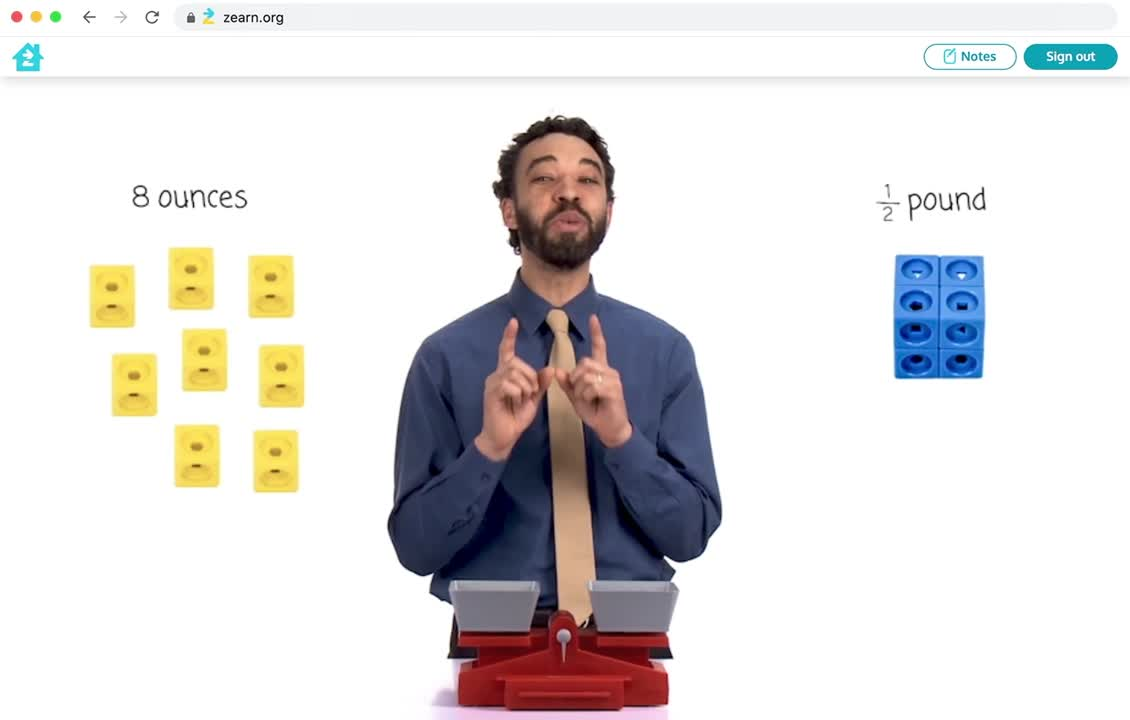
\includegraphics{images/zearn-poster.jpg}

}

\caption{\label{fig-zearn-poster}Example of Teaching with Visual Models
on Zearn}

\end{figure}

The platform's structure facilitates a personalized learning experience
for students (see SI for a screenshot of the student portal), allowing
teachers to track student progress and make informed decisions (see
Figure~\ref{fig-class-report} for a sample class report). This structure
includes self-paced online lessons and small group instruction, a
rotational model that allows students to learn new grade-level content
in two ways: independently through engaging digital lessons, and in
small groups with their teacher and classmates. This dual approach
enables students to learn at their own pace, fostering a sense of
autonomy and self-directed learning.

\begin{figure}

{\centering 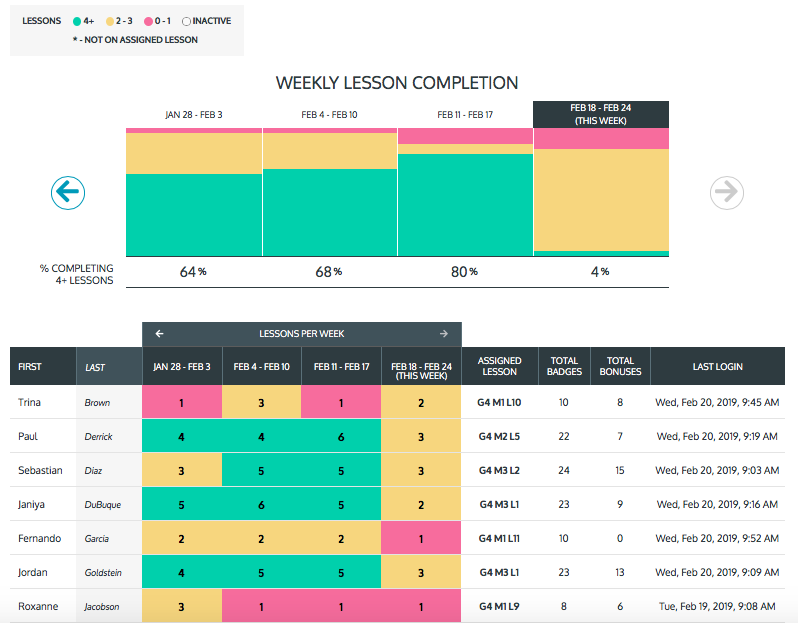
\includegraphics{images/class-report.png}

}

\caption{\label{fig-class-report}Sample Class Report}

\end{figure}

A key feature of Zearn is its badge system, which serves as a mechanism
for tracking student progress and motivating continued learning (see
Figure~\ref{fig-badges-screen}). Students earn badges upon mastery of
specific skills, providing a tangible representation of their
achievement. This system motivates students and provides teachers with
valuable data on student performance, informing their decision-making
process \citep{knudsen2020}. Zearn also incorporates notifications,
known as Tower Alerts, sent to teachers when a student struggles with a
specific concept. This feature allows teachers to provide timely support
and address learning gaps, enhancing the platform's capacity for
personalized learning.

\begin{figure}

{\centering 
\includegraphics{images/badges.PNG}

}

\caption{\label{fig-badges-screen}Badge System for Student Achievement}

\end{figure}

Another noteworthy aspect is the platform's professional development
component, which is available for schools with a paid account (see SI
for a sample training schedule). Teachers explore each unit or mission
through word problems, fluencies, and small group lessons, conducting
collaborative analysis of student work and problem-solving strategies.
This professional development revolves around each mission's big
mathematical idea, visual representations to scaffold learning, and
strategies to address unfinished learning from prior grades and
preparation for future learning \citep{morrison2019}.

In order to model interesting behavioral patterns, we focus our analysis
on the teachers who most likely take advantage of a wide range of
resources on the platform. Thus, we select teachers who consistently use
the platform and work in traditional school settings.

The platform's integrated approach to math teaching and learning,
connecting a print- and software-based curriculum with a rotational
classroom model, professional development, and classroom- and
school-level reports on student learning, provides a comprehensive data
set for analysis. The variables of interest in this study have been made
available by the Zearn team and include (1) teacher effort (as measured
by a gamut of actions), (2) lesson completion (badges), (3) student
performance (tower alerts), and the (4) time teachers and students spend
on the platform.

\hypertarget{research-questions}{%
\subsection{Research Questions}\label{research-questions}}

We propose the following research questions to explore the complex
dynamics of teacher behavior, the role of reinforcement learning in
modeling these behaviors, and the subsequent impact on student
achievement. We hope to shed light on the potential of reinforcement
learning for understanding human behavior in field data.

1. Characterizing Teacher Behavior: Which reinforcement learning model
most accurately characterizes the behavior of teachers in the context of
Zearn Math? What insights about teacher behavior do these differences in
model fit bring?

2. Impact of RL Parameters on Teacher Behavior and Student Achievement:
How do the parameters of reinforcement learning models vary with teacher
behavior? What effects do these variations have on student achievement?

3. Influence of Teacher Background, Training, and Experience: How do
factors such as teacher background, training, and experience influence
their adaptation to and implementation of the Zearn Math curriculum? How
can these factors be effectively incorporated into the reinforcement
learning model to provide a more comprehensive understanding of teacher
behavior and its impact on student outcomes?

\hypertarget{theory}{%
\section{Theory}\label{theory}}

\hypertarget{education-production-function}{%
\subsection{Education production
function}\label{education-production-function}}

Previous research has explored how teacher effort affects student
achievement. In particular, economists have studied the ``education
production function,'' in which educational outcomes are a function of
various inputs, including teacher effort, student effort, school
resources, and family background \citep{hedges1994}. This function
serves as a theoretical framework for understanding how different
factors contribute to educational achievement and how interventions can
be designed to improve outcomes.

One of the key inputs in the education production function is teacher
effort, as teachers play a crucial role in shaping students' learning
experiences and outcomes. Their effort, which encompasses their time,
energy, dedication, and instructional strategies, can significantly
influence students' academic achievement \citep{rivkin2005}. However,
measuring teacher effort and its impact on student outcomes can be
challenging due to the complex and multifaceted nature of teaching.

To address this challenge, researchers have employed various strategies
to identify the effects of teacher effort on student achievement. One
common approach is to manipulate the conditions under which teachers
operate, thereby changing the levels of teacher effort. For instance,
Duflo, Dupas, and Kremer (2011) \citep{duflo2011} conducted a randomized
controlled trial in Kenya to examine the effects of tracking, a practice
of grouping students based on their ability levels. Tracking has been a
prominent tool in the sociology of education and assumes that teacher
inputs will depend on the ability level of the students. This tailoring
of teaching strategies and content potentially enhances the instructor's
effectiveness.

However, traditional social science approaches to studying the education
production function often lack the flexibility to account for changes in
context and experience and individual-level differences. Reinforcement
learning (RL) offers a promising alternative approach. RL models
incorporate a flexibility term (i.e., a learning rate) that allows for
changes in behavior with experience, and an exploration versus
exploitation term (e.g., inverse temperature) that captures individual
differences in decision-making strategies. Furthermore, the RL framework
inherently accounts for the process of learning about rewards, making it
a flexible and dynamic tool for studying teacher behavior
\citep{sutton2018}.

\hypertarget{reinforcement-learning-to-capture-patterns-in-repeated-behavior}{%
\subsection{Reinforcement Learning to Capture Patterns in Repeated
Behavior}\label{reinforcement-learning-to-capture-patterns-in-repeated-behavior}}

In RL, an agent learns to make decisions over time to maximize a
cumulative reward. At the heart of RL is the concept of a policy, which
is a mapping from states to actions, or more commonly, a probability
distribution over actions \citep{sutton2018}. The agent's goal is to
learn an optimal policy, which maximizes the expected cumulative reward,
even when the parameters of the environment are not known a priori.

The application of RL in the context of education and teaching is not
new. One of the pioneers in the field of Markov decision processes,
Ronald Howard, attempted to apply his mathematical framework to
instruction theory as early as 1960 \citep{howard1960}. Later, in 1972,
Richard Atkinson proposed a theory of instruction that encapsulates the
key components of a Markov decision process, including states, actions,
transition probabilities, reward functions, and a time horizon
\citep{atkinson1972}. In Atkinson's framework, actions are instructional
activities (e.g., assigning problem sets) that can change a given state
(e.g., student learning level). These changes of states can yield
rewards minus the associated cost of the action. For example, a teacher
may be rewarded by an increase in the knowledge or skill of a student,
but such reward must be balanced with its associated effort (e.g., labor
cost). Atkinson and colleagues continued to test many parametrizations
of this idea, contributing significantly to the development of RL theory
in the context of education (see \citep{doroudi2019} for a full review).

More recently, RL models have been used in the psychology of habit to
explain learning and reward association. One common approach in human
studies is to apply the ``multi-armed bandit'' task. In this type of
experiment, participants are presented with multiple actions, each with
an unknown payoff. The subject's goal is to learn the best outcome
through trial and error. In the beginning, the reward-action
relationships are unknown, so the participant must explore or sample
from each action \citep{sutton2018}. This exploration-exploitation
trade-off is a central theme in RL and has the potential to provide
valuable insights into how students learn and make decisions over time.

\hypertarget{why-reinforcement-learning}{%
\subsubsection{Why Reinforcement
Learning?}\label{why-reinforcement-learning}}

Before presenting these models, we argue for the usefulness of RL in our
setting. Unlike traditional economic models that map teacher effort to
student outcomes through a time-fixed education production function, RL
allows us to model teacher behavior as a flexible, evolving process that
can change week by week. The RL framework is inspired by the way animals
learn from their experiences, with an agent representing a
decision-maker that performs actions in an environment and receives
observations and rewards in return. In the RL paradigm, teachers are
modeled as agents that interact with their environment (the classroom),
making decisions (actions) based on their current understanding of the
environment (state) and the feedback they receive (rewards). This
interaction can be represented as:

\[
\text{Agent} \xrightarrow[\text{Actions}]{\text{Performs}} \text{Environment} \xrightarrow[\text{Observations, Rewards}]{\text{Provides}} \text{Agent}
\]

In the context of predicting repeated behavior, we can use RL algorithms
to model the decision-making process of individuals or groups, such as
teachers, by learning from the patterns in their actions and the
resulting outcomes. This approach allows us to model how individual
teachers learn the relationships between actions, states, and rewards,
thereby creating a typification of instructors. The RL framework's
flexibility and robustness make it adaptable to changes in the learning
environment and individual student needs. Furthermore, it allows for
incorporating a diverse range of state, action, and reward variables and
can be tailored to different educational contexts and objectives. RL
models can also capture the inherent uncertainty in the teaching
environment, providing a framework for making optimal decisions under
uncertainty. This feature is particularly relevant in the context of
teaching, where the effectiveness of a teaching strategy may not be
immediately apparent, and the optimal strategy may evolve as students'
understanding develops.

With RL, it then becomes possible to identify how teachers differ in
their learning and behavior and how these characteristics relate to
student outcomes. For example, teacher flexibility may be optimal in a
learning environment, but without estimation of individual parameters,
differentiating teachers would not be possible. Further, if a
policy-maker can shift these individual-level parameters, they can
affect student outcomes. These so-called ``counterfactual analyses'' can
be powerful tools in creating innovative interventions or nudges to
improve an outcome of interest. Finally, the RL model carries potential
beyond the goals of this study. For instance, it can learn the
associations between actions and rewards, allowing for automation of
certain instructional inputs; if a teacher often assigns an activity
under a certain state, the model could automate this action, freeing
some of the teacher's time.

\hypertarget{q-learning-model}{%
\subsubsection{Q-Learning Model}\label{q-learning-model}}

The first class of models we apply to our data is the so-called
Q-learning algorithm. Q-learning is a model-free reinforcement learning
algorithm designed to learn a policy, which tells an agent what action
to take under what circumstances \citep{watkins1992}. It does not
require a model of the environment (hence the connotation
``model-free''), and it can handle problems with stochastic transitions
and rewards without requiring adaptations. This model is inspired by the
so-called ``multi-armed bandit'' problem. In this paradigm, an agent has
a finite number of choices, each associate with a given reward. The
agent must simply learn to choose which action yields the highest
reward. Learning in this setting occurs by adjusting expectations and
minimizing ``surprises'' (i.e., prediction errors). Notice that this
setting does not require us to define a given state: in our simplest
model, Q-learning assumes that the best action in one week is the best
action at any other week. Thus, the model only prescribes an
action-reward relationship. The teacher here learns the value of logging
in regardless of the history of their classroom or students.

In the context of Q-learning, the agent interacts with the environment
to gain experience and uses this experience to update its knowledge
about the quality of particular actions, given the state of the
environment. This knowledge is represented in the Q-values, a prediction
of the future reward expected after taking an action in the current
state (which in our context can be compared to subjective value, or a
utility). The goal of Q-learning is to accurately learn these Q-values
by updating them iteratively \citep{rummery}.

The Q-learning model is based on the concept of a Q-function, which is a
function of both state and action, and represents the expected future
reward for taking a particular action in a particular state. The
Q-function is updated iteratively using the Bellman equation, which
expresses the value of a state-action pair in terms of the immediate
reward plus the discounted value of the best future state-action pair.

The Q-function, denoted as \(Q(s, a)\), is defined for all state-action
pairs \((s, a)\), where \(s\) is the state and \(a\) is the action. The
Q-function represents the expected return or future reward for taking
action \(a\) in state \(s\) following a certain policy \(\pi\). The
Q-function is updated iteratively using the Bellman equation, as
follows:

\begin{equation}\protect\hypertarget{eq-q-learn}{}{
Q(s, a) = Q(s, a) + \alpha \delta
}\label{eq-q-learn}\end{equation}

where \(\alpha\) is the learning rate, which determines how much the
Q-value is updated based \(\delta\), the reward prediction error. The
reward prediction error is the difference between the estimated Q-value
and the observed reward plus the discounted future Q-value. This error
is used to update the Q-value in the direction of the observed reward,
as follows:

\begin{equation}\protect\hypertarget{eq-RPE}{}{
\delta = r + \gamma \max_{a'} Q(s', a') - Q(s, a)
}\label{eq-RPE}\end{equation}

where:

\begin{itemize}
\item
  \(r\) is the immediate reward received after taking action \(a\) in
  state \(s\),
\item
  \(\gamma\) is the discount factor,
\item
  \(s'\) is the new state after taking action \(a\),
\item
  \(a'\) is the action to be taken in the new state \(s'\),
\item
  \(s\) is the current state,
\item
  \(a\) is the action taken,
\item
  \(\max_{a'} Q(s', a')\) is the maximum reward that can be obtained in
  the next state \(s'\),
\item
  \(Q(s, a)\) is the current estimate of the Q-value for action \(a\) in
  state \(s\).
\end{itemize}

The Q-learning algorithm uses this update rule to learn the Q-function
and, hence, the optimal policy. The agent starts with an initial
Q-function (which can be arbitrary) and then updates the Q-values based
on the experiences it gathers from interactions with the environment.
The update rule is applied every time the agent transitions from a state
\(s\) to a state \(s'\) by taking an action \(a\) and receiving a reward
\(r\). The agent selects actions based on a policy derived from the
Q-values. A common choice is the softmax action selection method, which
is a way to balance exploration and exploitation. The softmax method
chooses actions probabilistically based on their Q-values. The softmax
function determines the probability of choosing a particular action and
is defined as follows:

\begin{equation}\protect\hypertarget{eq-softmax}{}{
P(a) = \frac{e^{Q(s, a)/\tau}}{\sum_{a'} e^{Q(s, a')/\tau}}
}\label{eq-softmax}\end{equation}

where:

\begin{itemize}
\item
  \(P(a)\) is the probability of choosing action \(a\),
\item
  \(Q(s, a)\) is the Q-value of action \(a\) in state \(s\),
\item
  \(\tau\) is a parameter known as the temperature, which controls the
  level of exploration,
\item
  the denominator is the sum over all possible actions \(a'\) of the
  exponential of their Q-values divided by the temperature.
\end{itemize}

The temperature parameter \(\tau\) controls the trade-off between
exploration and exploitation. When \(\tau\) is high, the agent explores
more because the action probabilities are more uniform. When \(\tau\) is
low, the agent exploits more because the action with the highest Q-value
is more likely to be chosen than the others. As the agent learns, it can
be beneficial to start with a high temperature to encourage exploration
and then gradually decrease it to favor exploitation of the learned
policy.

\hypertarget{state-free-vs.-state-based-models}{%
\subsubsection{State-Free vs.~State-Based
Models}\label{state-free-vs.-state-based-models}}

So far, we have defined state-based models incorporating the environment
into the Q-function. In state-free models, the Q-function, denoted as
\(Q(a)\), is solely a function of the action, \(a\). The environmental
state does not factor into the decision-making process. This simplifying
assumption can be beneficial in scenarios where the environmental state
exerts minimal influence on the outcome of the action. The agent learns
a global policy that is independent of the specific state. This approach
can be effective in environments with low state-action complexity or
when the state is difficult to define or observe \citep{sutton2018}. The
Q-value update function, therefore, simplifies to:

\begin{equation}\protect\hypertarget{eq-state-free}{}{
Q(a) = Q(a) + \alpha \left[ r(a) - Q(a) \right]
}\label{eq-state-free}\end{equation}

where:

\begin{itemize}
\item
  \(Q(a)\) is the current estimate of the Q-value for action \(a\),
\item
  \(\alpha\) is the learning rate,
\item
  \(r(a)\) is the immediate reward received after taking action \(a\).
\end{itemize}

In this equation, the term in the brackets, \(r(a) - Q(a)\), is the
reward prediction error. It represents the difference between the
observed reward and the current estimate of the Q-value. The Q-value is
updated in the direction of this error, scaled by the learning rate
\(\alpha\).

\hypertarget{the-kernel-function}{%
\subsubsection{The Kernel Function}\label{the-kernel-function}}

The kernel function is a mathematical tool used to measure the
similarity between different states or actions
\citep{ormoneit2002, domingues, liu}. In the context of the Q-learning
model with states and a kernel, the kernel function is used to compute a
weighted average of the rewards obtained in similar state-action pairs
in the past. This allows the model to generalize from past experience
and to make more informed decisions about future actions.

\hypertarget{the-actor-critic-model}{%
\subsubsection{The Actor-Critic Model}\label{the-actor-critic-model}}

The next model we attempt to fit divides the action selection and action
evaluation tasks into two components: the ``actor'' and the ``critic''
\citep{sutton2018b}. This division theoretically allows for more
efficient learning, as the critic guides the actor's learning process.

The ``actor'' in this model selects actions based on a policy function,
denoted as \(\pi(a|s)\), which maps states to actions, determining the
probability of taking each action in each state. The actor aims to learn
an optimal policy that maximizes the expected cumulative reward. In our
setting, we set the policy as a softmax function over action
preferences:

\[
\pi(a|s) = \frac{e^{h(a, s)}}{\sum_{a'} e^{h(a', s)}}
\]

where \(h(a, s)\) is the preference for action \(a\) in state \(s\).

The ``critic,'' on the other hand, evaluates the actions taken by the
actor by learning a value function, denoted as \(V(s)\). Given the
actor's current policy, the critic estimates the expected cumulative
reward from each state. The critic's feedback, in the form of the value
function, guides the actor's learning. We update the value function
based on the Temporal Difference (TD) error, a measure of the difference
between the estimated and actual return:

\[
\delta = r + \gamma V(s') - V(s)
\]

where \(r\) is the reward, \(\gamma\) is the discount factor, \(s'\) is
the new state, and \(s\) is the current state.

This separation of action selection and evaluation distinguishes the
Actor-Critic model. In Q-learning, a single Q-function selects and
evaluates actions. Conversely, in the Actor-Critic case, the actor
updates its policy to increase the probability of actions that lead to
higher-than-expected returns and decrease the probability of actions
that lead to lower-than-expected returns.

\hypertarget{applying-rl-models-to-the-zearn-context}{%
\section{Applying RL Models to the Zearn
Context}\label{applying-rl-models-to-the-zearn-context}}

In this section, we propose an application of the Reinforcement Learning
(RL) algorithms for modeling teacher decision-making within the Zearn
platform.

Consider a typical teaching scenario: the state is the students' current
progress in the class, and the actions are a range of pedagogical
strategies, such as assigning additional practice, providing
personalized feedback, or adjusting lesson plans. Some relevant reward
variables include improved student performance, increased student
engagement, or reduced learning gaps. We represent this interaction as:

\begin{equation}\protect\hypertarget{eq-zearn-RL}{}{
State (S) \xrightarrow[\text{Action (A)}]{\text{Teacher Decides}} New State (S') \xrightarrow[\text{Reward (R)}]{\text{Resulting Outcome}} \text{Feedback}
}\label{eq-zearn-RL}\end{equation}

In the Zearn context, we define the decision process as follows:

\begin{enumerate}
\def\labelenumi{\arabic{enumi}.}
\item
  Agents are the teachers.
\item
  Actions include the time spent on the platform and the choice to apply
  specific pedagogical strategies.
\item
  The environment is the Zearn platform with its students.
\item
  The state is the week-over-week change in Tower Alerts.
\item
  The reward is a linear function of the number of badges earned.
\end{enumerate}

Mathematically mapping the agent-environment interaction is flexible,
with many models potentially satisfying our initial assumptions. We
approach this problem as a competition of models, selecting a set of
models applicable to our setting, fitting them to the data, and
comparing their performances.

\hypertarget{state-free-q-learning-model}{%
\subsection{State-Free Q-Learning
Model}\label{state-free-q-learning-model}}

We use the Q-learning model to predict the actions of teachers based on
their past actions and the rewards they received.

The Q-value for a given state \(s\) and action \(a\) is updated based on
the reward prediction error \(\delta\):

\[
Q(a) = Q(a) + \alpha \left( \gamma (\text{Badges}_t - \text{cost}(a)) - Q(a) \right)
\]

where

\begin{itemize}
\tightlist
\item
  \(\alpha\) is the learning rate,
\item
  \(\gamma\) is the discount rate,
\item
  \(\text{Badges}_t\) is the immediate reward received after taking
  action \(a\) in state \(s\),
\item
  \(\text{cost}(a)\) is the cost associated with action \(a\),
\item
  \(Q(a)\) is the current estimate of the Q-value for action \(a\).
\end{itemize}

The probability of choosing a particular action is determined by the
softmax function and is defined as follows:

\[
P(a) = \frac{e^{Q(a)/\tau}}{\sum_{a'} e^{Q(a')/\tau}}
\]

where:

\begin{itemize}
\tightlist
\item
  \(P(a)\) is the probability of choosing action \(a\),
\item
  \(Q(a)\) is the Q-value of action \(a\),
\item
  \(\tau\) is a parameter known as the temperature, which controls the
  level of exploration.
\end{itemize}

Note that the reward is assumed to be a linear function of the number of
badges earned, with the learning rate \(\alpha\) as the multiplier and
the cost as the constant subtracted from the reward. We interpret each
of these parameters as follows:

\begin{itemize}
\item
  Reward: A linear function of the number of badges earned, indicating
  that the more badges a teacher earns, the higher the reward. The
  learning rate determines how quickly the teacher updates their
  Q-values in response to new information, while the cost represents the
  perceived effort or inconvenience associated with the action.
\item
  Cost: The perceived effort or inconvenience associated with the
  action, such as the effort required to complete a particular task or
  the inconvenience of deviating from a preferred teaching method.
\item
  Learning rate (\(\alpha\)): The extent to which the newly acquired
  information will override the old information. A factor of 0 will make
  the agent not learn anything.
\item
  Discount rate (\(\gamma\)): The degree to which future rewards are
  discounted compared to immediate rewards. A high discount rate means
  that future rewards are considered almost as valuable as immediate
  rewards, which encourages long-term planning. A low discount rate
  means that immediate rewards are much more valuable than future
  rewards, which encourages short-term thinking.
\item
  Inverse temperature (\(\tau\)): The degree of randomness in the choice
  behavior. A high inverse temperature means that the agent is more
  likely to choose the action with the highest expected reward, while a
  low inverse temperature means that the agent is more likely to choose
  actions randomly. This parameter can be interpreted as a measure of
  the agent's confidence in its Q-values, reflecting the trade-off
  between exploration (trying out new actions) and exploitation
  (sticking to known beneficial actions).
\end{itemize}

\hypertarget{state-based-q-learning-model}{%
\subsection{State-Based Q-Learning
Model}\label{state-based-q-learning-model}}

In this model, the state \(s\) represents the current situation or
context in which the teacher decides. The state could include factors
such as the students' current performance level. The state-dependent
model is particularly relevant in teaching, where the effectiveness of a
given strategy may depend on the specific circumstances of the class.
Here, the Q-value for a given state \(s\) and action \(a\) is:

\[ Q(s, a) = Q(s, a) + \alpha \left( \gamma (\text{Badges}_t - \text{cost}(a)) - Q(s, a) \right) \]

where:

\begin{itemize}
\tightlist
\item
  \(\alpha\) is the learning rate,
\item
  \(\gamma\) is the discount rate,
\item
  \(\text{Badges}_t\) is the immediate reward received after taking
  action \(a\) in state \(s\),
\item
  \(\text{cost}(a)\) is the cost associated with action \(a\),
\item
  \(Q(s, a)\) is the current estimate of the Q-value for action \(a\) in
  state \(s\).
\end{itemize}

Like the state-free model, the softmax function determines the
probability of choosing a particular action.

\hypertarget{the-kernel-function-1}{%
\subsection{The Kernel Function}\label{the-kernel-function-1}}

We anticipate that the reward associated with a given action may be
delayed, reflecting the time it takes for the effects of an action to
manifest. For instance, teachers might spend the first week of each
month planning activities on the platform, with the rewards of these
actions becoming apparent in subsequent weeks. To capture this temporal
aspect of teacher behavior, we employ a kernel function that
incorporates a measure of similarity between the current and past
state-action pairs, modulated by a discount factor that accounts for the
delay in reward. The kernel function is defined as the Jaccard
similarity, as follows:

\[
K(t, t') = 0.5 \cdot \text{I}(a_t = a_{t'}) \cdot \left[ 1 + \text{I}(s_t = s_{t'})\right]
\]

where:

\begin{itemize}
\tightlist
\item
  \(K(t, t')\) is the kernel function,
\item
  \(t\) and \(t'\) are the current and past time steps (weeks),
  respectively,
\item
  \(\text{I}(\cdot)\) is the indicator function, which equals 1 if the
  condition inside the parentheses is true and 0 otherwise,
\item
  \(a_t\) and \(a_{t'}\) are the choices made at the current and past
  time steps, respectively,
\item
  \(s_t\) and \(s_{t'}\) are the states at the current and past time
  steps, respectively.
\end{itemize}

\hypertarget{kernel-based-reinforcement}{%
\subsubsection{Kernel-Based
Reinforcement}\label{kernel-based-reinforcement}}

We use the kernel function to compute a weighted average of past rewards
(kernel reward), which updates the Q-value for the current state-action
pair. The kernel reward is:

\[
R_K = \frac{\sum_{t' = 1}^{T} K(t, t') \cdot \gamma^{(t - t')}  \text{Badges}_{t'}}{\sum_{t' = 1}^{T} K(t, t')}
\]

where:

\begin{itemize}
\tightlist
\item
  \(R_K\) is the kernel reward,
\item
  \(\gamma\) is the discount rate,
\item
  \(\text{Badges}_{t'}\) is the number of badges earned at the past time
  step \(t'\),
\item
  \(T\) is the number of lags in the kernel.
\end{itemize}

Subsequently, the Q-value for the current state-action pair is updated:

\[
Q(s, a) = Q(s, a) + \alpha \left( R_K - \text{cost}(a) - Q(s, a) \right)
\]

\hypertarget{dynamic-analysis-lau-glimcher-2005}{%
\subsection{Dynamic Analysis (Lau \& Glimcher,
2005)}\label{dynamic-analysis-lau-glimcher-2005}}

In order to determine the number of lags in the kernel, we apply the
Dynamic Analysis method, as proposed by \citep{lau2005}. The Dynamic
Analysis method is based on the premise that both past reinforcers and
past choices significantly influence an individual's choices on each
trial. It is a powerful tool for understanding choice behavior in the
context of reinforcement learning. This method is particularly useful in
tasks where reinforcement contingencies vary within a session, as it
allows for the analysis of behavior at a granular, response-by-response
level, while also providing insights into behavior averaged over
multiple trials. It also implies that the ratio of responses to
different alternatives matches the ratio of reinforcements obtained from
these alternatives. The method allows for the prediction of response
rate using weighted sums of past reinforcers, a technique that has been
applied to predict choice allocation in concurrent schedules on both
short (response-by-response) and longer (within and between sessions)
time scales.

Based on logistic regression, the model captures the linear combination
of past reinforcers and choices on each trial, as defined by:

\[
\begin{aligned}\log \left(\frac{p_{R, i}}{p_{L, i}}\right)= & \sum_{j=1} \alpha_{ j}( r_{R, i-j}-r_{L, i-j}) \\& +\sum_{j=1} \beta_{j} (c_{R, i-j}-c_{L, i-j})+\gamma,\end{aligned}
\] where \(p\) is the probability of choice \(c\) (\(R\), right or
\(L\), left) at time \(i\) as a function of the rewards, \(r\), and
choices for every time point \(i-j\) in the history.

A key aspect of Dynamic Analysis is its focus on local variations in
behavior and how these relate to local variations in reinforcer history
and behavioral history. This local focus allows for the identification
of patterns and trends that may be obscured when looking at behavior on
a larger scale. For example, the method can reveal a tendency to
alternate between choices in the short term, while also showing a
longer-term tendency to persist with the more frequently chosen
alternative.

The Dynamic Analysis method also allows for the quantitative assessment
of the relative effects of past reinforcers and choices. This is
achieved by including covariates (\(\alpha, \beta\)) for past choices in
the analysis, which can reveal patterns such as a fix-and-sample pattern
of choice, where there is a tendency to persist on the rich alternative
with brief visits to the lean alternative.

In terms of the weighting of past reinforcers and choices, the Dynamic
Analysis method suggests that the effects of these factors decay over
time. This is represented by a decay function, which can take the form
of an exponential or hyperbolic function, depending on the specific
characteristics of the task and the behavior of the individual.

\hypertarget{dynamic-analysis-in-the-zearn-context}{%
\subsubsection{Dynamic Analysis in the Zearn
context}\label{dynamic-analysis-in-the-zearn-context}}

In the context of the Zearn dataset, we implement the Dynamic Analysis
method to understand the temporal dependencies and complex interactions
between teacher actions, student outcomes, and the learning environment.
The method is applied to a panel data model, which allows for the
inclusion of both time-invariant and time-varying variables, and
accounts for individual-specific effects. The key variables in the model
are the rewards and choices. In this context, the rewards are
represented by Badges per active student in a given week. The choices
are represented by Teacher Minutes or the components from our
dimensionality reduction. The model also includes lagged versions of
these variables, which capture the effects of past rewards and choices
on current choices. The lag period ranges from 1 week to 8 weeks,
allowing for the examination of the effects of past rewards and choices
over different time horizons.

The model can be represented by the following equation:

\[
y_{it} = \beta_0 + \sum_{j=1}^{L} \beta_{1j} y_{it-j} + \beta_2 x_{it} + \sum_{j=1}^{L} \beta_{3j} x_{it-j} + u_i + \epsilon_{it}
\]

where:

\begin{itemize}
\tightlist
\item
  \(y_{it}\) is the dependent variable (teacher minutes or method
  component) for individual \(i\) at time \(t\),
\item
  \(y_{i t-j}\) is the dependent variable lagged by \(j\) periods,
\item
  \(x_{it}\) is the independent variable (badges per active user) for
  individual \(i\) at time \(t\),
\item
  \(x_{i t-j}\) is the independent variable lagged by \(j\) periods,
\item
  \(u_i\) is the individual-specific effect,
\item
  \(\epsilon_{it}\) is the error term, and
\item
  \(L\) is the number of lag periods.
\end{itemize}

The coefficients \(\beta_1j\) and \(\beta_3j\) capture the effects of
past choices and rewards, respectively, lagged by \(j\) periods, on
current choices. The sum over \(j\) from \(1\) to \(L\) represents the
inclusion of lagged variables for all lag periods from 1 week to 8
weeks.

The Dynamic Analysis method offers several advantages in the context of
the Zearn dataset. First, it captures the temporal dependencies and
complex interactions between teacher actions, student outcomes, and the
learning environment. This allows for a more nuanced understanding of
the factors that influence teacher behavior on the platform.

Second, the method allows for the identification of a kernel that best
describes the temporal dynamics of the data. This kernel, represented by
the lagged variables in the model, captures how far back rewards and
past actions matter. This can provide valuable insights into the
temporal scope of the effects of rewards and actions, and can inform
strategies for influencing teacher behavior on the platform.

\hypertarget{the-actor-critic-model-1}{%
\subsection{The Actor-Critic Model}\label{the-actor-critic-model-1}}

In this model, we estimate several variables: the cost in badge-units
for each component, the discount rate (\(\gamma\)), and step-sizes
(\(\alpha_v\) and \(\alpha_\pi\)). These step-sizes are similar to
learning rates, as they determine the extent to which the model updates
the weights for the value and policy functions, respectively.

Our Actor-Critic model maintains two sets of parameters: the weights
\(w_a\) that parameterize the value function (the critic) and the
parameters \(\theta_a\) that define the policy (the actor). The weights
and policy are updated based on the prediction error \(\delta\). The
equations for updating the weights and policy are as follows:

\[
w_a = w_a + \alpha_{v} \cdot \delta \cdot S \\
\theta_a = \theta_a + \alpha_{\pi} \cdot \delta \cdot S
\]

where \(w_a, \theta_a\) are the vectors of policy and value weights,
respectively, for action \(a\), and \(S\) is a vector that characterizes
the current state, defined as
\(S = \begin{bmatrix} 1 \\ \text{Tower Alerts}_t - \text{Tower Alerts}_{t-1} \end{bmatrix}\).

We define the parameterized policy as
\(\text{Prob}(a)=\text{Logit}^{-1}(\theta_a \cdot S)\), the values of
each state as \(v(S,a) = w_a \cdot S\), and prediction error \(\delta\)
as the difference between the actual outcome and the estimated value of
the state-action pair:

\[
\delta = (\text{Badges}_{t} - \text{cost}(a)) - \left( \gamma v(S,a) - v(S',a) \right)
\]

\hypertarget{hierarchical-models}{%
\subsection{Hierarchical Models}\label{hierarchical-models}}

Our dataset comprises of classrooms spanning a period of around 40
weeks. Given the limited amount of data per classroom, individual-level
estimation using maximum likelihood estimation would yield noisy
results. Although group-level estimation provides reliable estimates, it
overlooks individual differences, which are crucial to our analysis.

To address this, we employed a hierarchical Bayesian analysis, which
allows for information pooling across individuals while accommodating
individual differences. In this approach, individual-level parameters
are functions of group-level hyperparameters, and this anchoring
enhances our power by assuming commonalities among individuals
\citep{ahn2017}. A notable feature of this estimation technique is that
the extent of pooling is reflected in the hyperparameter variance.
Strong pooling corresponds to low hierarchical variance, and vice versa
for weak pooling.

\hypertarget{data}{%
\section{Data}\label{data}}

Our data from the Zearn platform follows a time-series structure,
spanning across an academic year, with the unit of analysis being the
classroom-week. This level of granularity enables us to capture the
temporal dynamics of teacher-student interactions and their subsequent
influence on student achievement. In particular, we can model the
decision-making process of teachers as they allocate their time and
effort on the Zearn platform weekly and how these decisions translate
into student outcomes, measured by the completion of lessons or
``badges.''

Geographically, the data encompasses a diverse range of schools in
Louisiana. This geographical focus provides a fascinating context for
our study, given the state's unique educational landscape and the
widespread adoption of the Zearn platform across its schools. However,
the insights derived from this study potentially have broader
implications, extending beyond the confines of Louisiana, given the
universal teaching and learning principles underpinning our analysis.

Figure~\ref{fig-teachers-map} depicts the geographical distribution of
teachers using the Zearn platform across various parishes in Louisiana.
This map visually represents the number of teachers per parish,
revealing a heterogeneous distribution of Zearn usage across Louisiana,
with certain parishes demonstrating a higher concentration of teachers.
The map also highlights the top five cities with the highest number of
teachers using Zearn.

\begin{figure}

{\centering \includegraphics{zearn_files/figure-pdf/fig-teachers-map-1.pdf}

}

\caption{\label{fig-teachers-map}Geographical distribution of teachers
across various parishes in Louisiana, and the top 5 cities with the
highest number of teachers.}

\end{figure}

\hypertarget{descriptive-collection-and-preprocessing}{%
\subsection{Descriptive Collection and
Preprocessing}\label{descriptive-collection-and-preprocessing}}

Zearn provided administrative data for teachers and students at a
granular level. Teacher data was time-stamped by the second and included
the time spent on the platform and the specific actions taken. Note
that, although extensive, the set of actions was not comprehensive. On
the other hand, student data was aggregated at the classroom-week level
due to data privacy considerations. This aggregation included our
variables of interest: (1) teacher effort (weekly time spent on the
Zearn platform, in minutes), (2) student achievement (student lesson
completion or ``badges''), and (3) level of student struggle (tower
alerts). These variables form the basis of our reinforcement learning
models, providing a comprehensive view of the dynamics of
teacher-student interactions on the Zearn platform.

The dataset represents various aspects of Zearn schools including
identifiers, usage data, and demographic information. It contains
information for 22153 classrooms and 13921 teachers, with an average of
20 students per classroom.

The school summary statistics, as presented in Table~\ref{tbl-summary},
provide a snapshot of the schools' characteristics. The table reveals
the average number of teachers, students, and weeks of data per school.
Table~\ref{tbl-proportions} presents the proportions of schools across
different poverty levels, income brackets, and other variables, such as
the percentage of charter schools and schools with paid accounts. These
proportions provide insights into the socio-economic context of the
schools in the dataset, which is crucial for understanding the external
factors that may influence teacher effort and student achievement.

\hypertarget{tbl-summary}{}
\begin{longtable}{l|rrrr}
\caption{\label{tbl-summary}Summary statistics for the schools }\tabularnewline

\toprule
\multicolumn{1}{l}{} & Mean & Standard Deviation & Minimum & Maximum \\ 
\midrule
Teachers & $12.08$ & $11.84$ & $1$ & $72$ \\ 
Students\_Total & $268.72$ & $279.49$ & $1$ & $3,289$ \\ 
Weeks\_Total & $9.30$ & $7.16$ & $1$ & $39$ \\ 
\bottomrule
\end{longtable}

\hypertarget{tbl-proportions}{}
\begin{longtable}{l|r}
\caption{\label{tbl-proportions}Proportions of different variables. }\tabularnewline

\toprule
\multicolumn{1}{l}{} & Proportions \\ 
\midrule
\textbf{Poverty Level} &  \\ 
0-40\% (Low) & 20.12\% \\ 
40-75\% (Mid-High) & 53.44\% \\ 
75\%+ (High) & 20.52\% \\ 
\textbf{Income} &  \\ 
\$1--27,999 & 5.12\% \\ 
\$28K-31,999 & 5.81\% \\ 
\$32K-34,999 & 7.39\% \\ 
\$35K-36,999 & 4.61\% \\ 
\$37K-38,999 & 3.52\% \\ 
\$39K-40,999 & 2.55\% \\ 
\$41K-42,999 & 5.34\% \\ 
\$43K-44,999 & 3.66\% \\ 
\$45K-47,999 & 7.11\% \\ 
\$48K-51,999 & 18.48\% \\ 
\$52K-54,999 & 4.16\% \\ 
\$55K-59,999 & 2.95\% \\ 
\$60K-64,999 & 9.1\% \\ 
\$65K-69,999 & 4.02\% \\ 
\$70K-80,999 & 8.8\% \\ 
\$81K-93,999 & 2.94\% \\ 
\$94K+ & 1.62\% \\ 
\textbf{Other} &  \\ 
Charter\_Schools & 7.01\% \\ 
Schools\_with\_Paid\_Account & 71.04\% \\ 
\bottomrule
\end{longtable}

\hypertarget{temporal-dynamics-of-student-engagement}{%
\subsubsection{Temporal Dynamics of Student
Engagement}\label{temporal-dynamics-of-student-engagement}}

The total number of weeks of data per classroom, as shown in
Figure~\ref{fig-classroom-weeks}, reveals that the distribution of the
number of weeks is bimodal, with one mode representing classrooms with
less than 3 to 4 months of data and the other mode representing
classrooms with four months or more. The classrooms with less than 16
weeks of data are color-coded in red and are excluded from the analysis.

Figure~\ref{fig-logins-week} illustrates the total number of student
logins over time, offering a dynamic view of student engagement with the
Zearn platform. Notably, there are marked decreases in logins during
Thanksgiving and Christmas, as indicated by the text annotations on the
plot.

\begin{figure}

{\centering \includegraphics{zearn_files/figure-pdf/fig-classroom-weeks-1.pdf}

}

\caption{\label{fig-classroom-weeks}Total number of weeks of data per
classroom.}

\end{figure}

\begin{figure}

{\centering \includegraphics{zearn_files/figure-pdf/fig-logins-week-1.pdf}

}

\caption{\label{fig-logins-week}Total number of student logins over
time.}

\end{figure}

\hypertarget{variables-of-interest}{%
\subsection{Variables of interest}\label{variables-of-interest}}

Our Zearn data can be viewed as time-series (over the course of the
school year, \textasciitilde{} 40 weeks). We propose to analyze the
relationship between teacher effort and student achievement through
temporal dynamics in the data. For the implementation of RL models, we
need both an input (action) and an output (reward). For this purpose, we
first use teacher weekly log-ins (a binary variable, 0 = no log-ins and
1 = at least 1 log-in) as a quantifiable proxy for teacher effort. We
assume that teachers on Zearn are in control of this input variable, and
choosing how much time to allocate to the platform is central to this
decision process. Although these are not perfect proxies (e.g., they do
not account for time spent creating assignments and performing in person
instruction to students), it is one of the few directly quantifiable
information about teacher behavior available in the data. Further, we
use student lesson completion (badges completed) as a measure of student
effort level, given that Zearn emphasizes the importance of lesson
completion (instead of a grade, for example).

\hypertarget{teacher-actions}{%
\subsubsection{Teacher Actions}\label{teacher-actions}}

Another way of capturing teacher behavior is by analyzing their specific
actions when they use Zearn. The platform provides a wide range of
actions that teachers can take, including downloading resources,
engaging in different teaching methods or activities, and choosing how
much time they spend online. We can use these actions to create a more
nuanced picture of teacher behavior on the platform. provides a list of
the actions available in our data.

\begin{longtable}[]{@{}
  >{\raggedright\arraybackslash}p{(\columnwidth - 2\tabcolsep) * \real{0.3134}}
  >{\raggedright\arraybackslash}p{(\columnwidth - 2\tabcolsep) * \real{0.6866}}@{}}
\caption{List of Teacher Actions}\tabularnewline
\toprule\noalign{}
\begin{minipage}[b]{\linewidth}\raggedright
Variable
\end{minipage} & \begin{minipage}[b]{\linewidth}\raggedright
Description
\end{minipage} \\
\midrule\noalign{}
\endfirsthead
\toprule\noalign{}
\begin{minipage}[b]{\linewidth}\raggedright
Variable
\end{minipage} & \begin{minipage}[b]{\linewidth}\raggedright
Description
\end{minipage} \\
\midrule\noalign{}
\endhead
\bottomrule\noalign{}
\endlastfoot
Assessments Answer Key Download & Answer keys for assessments to
facilitate grading. \\
Assessments Download & Assessments to demonstrate understanding of the
material. \\
Course Guide Download & Overview of the content, objectives, and
structure of Zearn's PD courses. \\
Course Notes Download & Notes from Zearn's professional development (PD)
courses. \\
Curriculum Map Download & Comprehensive overview of the learning
objectives and content for each grade level. \\
Elementary Schedule Download & Schedule of elementary-level activities
in the Zearn curriculum. \\
Fluency Completed & Tracks completion of a fluency activity. \\
Grade Level Overview Download & Overview of the curriculum for a
specific grade level. \\
Guided Practice Completed & Tracks completion of the guided practice
portion of a Zearn lesson. \\
Kindergarten Activity Completed & Tracks completion of a specific
activity in the Kindergarten curriculum. \\
Kindergarten Mission Download & A specific learning mission in the
Kindergarten curriculum. \\
Kindergarten Schedule Download & Detailed schedules for Kindergarten to
help teachers plan their instruction. \\
Mission Overview Download & Overview of a specific learning mission in
the Zearn curriculum. \\
Number Gym Activity Completed & Tracks completion of a Number Gym
activity. \\
Optional Homework Download & Optional homework assignments for extra
practice. \\
Optional Problem Sets Download & Optional sets of problems for extra
practice. \\
Small Group Lesson Download & Lessons designed for completion in small
groups. \\
Student Notes and Exit Tickets Download & Notes taken during a lesson
and ``exit tickets,'' brief assessments at the end of a lesson. \\
Teaching and Learning Approach Download & Resources related to Zearn's
teaching and learning approach. \\
Tower Completed & Tracks completion of a ``Tower of Power'' activity in
a Zearn lesson. \\
Tower Stage Failed & Tracks failure of a stage in a ``Tower of Power''
activity. \\
Tower Struggled & Tracks struggles with a ``Tower of Power''
activity. \\
Whole Group Fluency Download & Activities for practicing fluency skills
as a whole group. \\
Whole Group Word Problems Download & Word problem activities completed
as a whole group. \\
\end{longtable}

\hypertarget{state-variables}{%
\subsubsection{State Variables}\label{state-variables}}

For this paper's second class of Reinforcement Learning models, we
require variables that can determine the state space of each week.
Experienced teachers suggest that they strongly focus on measures of the
level of difficulty encountered during the lessons. The Zearn platform
provides a measure of this kind, namely, ``Tower Alerts.'' If a student
is struggling in a given lesson, the platform automatically provides
scaffolded remediation (i.e., breaking the problems step by step), and
if they struggle multiple times in that same lesson, a ``Tower Alert''
is generated for their teacher. We use the previous week's average Tower
Alerts to measure the level of difficulty faced by the students.
Further, we include the previous week's average student time usage (in
minutes) as a state variable. Effectively, we assume that the value of a
given state (i.e., the week at hand) is a function of the previous
week's ``tower alerts'' and ``student minutes.''

\hypertarget{exclusion-criteria}{%
\subsection{Exclusion criteria}\label{exclusion-criteria}}

The raw data underwent rigorous preprocessing to ensure its suitability
for analysis. This process included performing log transformations on
our variables of interest (i.e., minutes, badges, and tower alerts) to
normalize their distributions. Given the diverse user base of Zearn, we
applied specific exclusion criteria to select teachers who most likely
come from traditional schools and classrooms that use the platform
consistently. We selected virtual classrooms with at least five active
students weekly, filtering out parents or tutors who may use Zearn
outside the classroom setting. We removed teachers with more than four
classrooms and those who logged in for less than 16 weeks. We excluded
classrooms in the 6th to 8th grades, as those are a small proportion of
our dataset. This deletion ensures a focus on traditional school
settings and consistent platform usage, minimizing bias from teachers
and schools that have not used Zearn consistently.

Table~\ref{tbl-summary-statistics} summarizes the refined dataset,
providing a snapshot of the key variables of interest. Their means and
standard deviations (SD) are computed for each grade level and overall
(across all grades).

\begin{table}

\caption{\label{tbl-summary-statistics}\textbf{?(caption)}}\begin{minipage}[t]{\linewidth}
\subcaption{\label{tbl-summary-statistics-1}}

{\centering 

\begin{longtable*}{lllll}
\toprule
Grade Level & Minutes per Student & Badges per Student & Tower Alerts per Lesson Completion & Minutes per Teacher \\ 
\midrule
**Overall**, N = 114,681 & 84 (57) & 1.09 (0.57) & 0.33 (0.33) & 3.22 (1.85) \\ 
**Kindergarten**, N = 4,982 & 44 (38) & 1.48 (0.72) & 0.04 (0.19) & 1.91 (1.65) \\ 
**1st**, N = 17,240 & 84 (51) & 1.16 (0.52) & 0.31 (0.26) & 3.05 (1.82) \\ 
**2nd**, N = 21,910 & 87 (56) & 1.13 (0.54) & 0.27 (0.27) & 3.11 (1.81) \\ 
**3rd**, N = 22,605 & 86 (56) & 1.11 (0.56) & 0.32 (0.30) & 3.37 (1.86) \\ 
**4th**, N = 23,718 & 87 (60) & 1.02 (0.57) & 0.38 (0.34) & 3.41 (1.83) \\ 
**5th**, N = 24,226 & 86 (61) & 1.00 (0.55) & 0.43 (0.39) & 3.40 (1.83) \\ 
**6th**, N = 0 & NA (NA) & NA (NA) & NA (NA) & NA (NA) \\ 
**7th**, N = 0 & NA (NA) & NA (NA) & NA (NA) & NA (NA) \\ 
**8th**, N = 0 & NA (NA) & NA (NA) & NA (NA) & NA (NA) \\ 
\bottomrule
\end{longtable*}

}

\end{minipage}%

\end{table}

\hypertarget{visualizing-relationships-between-variables}{%
\subsection{Visualizing Relationships Between
Variables}\label{visualizing-relationships-between-variables}}

We begin to unveil the intricate relationships among the variables under
consideration through a comprehensive correlation analysis, as depicted
in Figure~\ref{fig-corr}. This correlation matrix elucidates the
magnitude and direction of associations among variables such as badges
earned, minutes spent per student, tower alerts, the number of students,
and teacher minutes. These interconnections inform the construction of
our reinforcement learning models by suggesting the influence of teacher
effort on student achievement. In this correlation matrix, each cell
represents the Spearman correlation coefficient between a pair of
variables. The color and size of the circles in each cell reflect the
strength and direction of the correlation, with blue indicating positive
correlations and red indicating negative correlations. The histograms
along the diagonal provide a visual representation of the distribution
of each variable.

\begin{figure}

{\centering \includegraphics{zearn_files/figure-pdf/fig-corr-1.pdf}

}

\caption{\label{fig-corr}Correlation coefficients between variables
after log transformation}

\end{figure}

\hypertarget{dimensionality-reduction}{%
\subsection{Dimensionality Reduction}\label{dimensionality-reduction}}

To capture the complex decision-making processes and trade-offs made by
teachers, we employed a Principal Component Analysis (PCA), a
Nonnegative Matrix Factorization (NMF), and an autoencoder (AE). We
chose these methods as candidates to condense the multifaceted nature of
our variables, including Teacher Minutes, Teacher Sessions, and the set
of teacher actions.

While PCA is a widespread technique, it is only appropriate for some
datasets or research questions. PCA assumes the data follows a Gaussian
distribution, which may not always hold \citep{jolliffe2016}. Further,
PCA is an unsupervised method that only considers the input data
structure and not the associated target variables or labels. On the
other hand, methods like NMF and autoencoders offer different
advantages. NMF, for instance, imposes a non-negativity constraint,
which makes its components easier to interpret in many contexts,
especially when the data elements represent quantities that cannot be
negative, such as counts or frequencies. NMF also tends to produce a
more parts-based, sparse representation of the data, which can be more
interpretable in some cases \citep{lee1999}. Autoencoders are a type of
neural network that can model more complex, non-linear relationships in
the data. They can also be trained in a supervised manner to learn a
reduced-dimension representation specifically optimized for predicting a
target variable, leading to improved performance in subsequent
predictive modeling tasks \citep{goodfellow2016}.

By trying different techniques, we can explore these different
trade-offs and potentially discover a reduced-dimension representation
better suited to our specific dataset and research question than PCA
alone would provide. This approach aligns with the principle of
methodological triangulation, which suggests that using multiple methods
can help to overcome the limitations of any single method and provide a
more robust and comprehensive understanding of the data.

The Nonnegative Matrix Factorization (NMF) operates as follows:

The original matrix is a detailed description of all the teachers'
behaviors. Each row in the matrix represents a unique teacher, and each
column represents a specific behavior or action the teacher might take.
The entry in a specific row and column corresponds to the frequency of
that behavior for that particular teacher.

After the NMF, we have two matrices:

\begin{enumerate}
\def\labelenumi{\arabic{enumi}.}
\tightlist
\item
  Basis Matrix (W): This matrix represents underlying behavior patterns.
  Each column is a ``meta-behavior'' or a group of behaviors occurring
  together.
\item
  Mixture Matrix (H): This matrix shows the extent to which each
  ``meta-behavior'' is present in each teacher. Each entry in this
  matrix represents the contribution of a ``meta-behavior'' to a
  particular teacher's behaviors.
\end{enumerate}

By looking at these matrices, we can identify underlying patterns of
behaviors (from the basis matrix) and see how these patterns are mixed
and matched in different teachers (from the mixture matrix).

We first scale the data such that all features are in the range {[}0,
1{]}, then we create training (80\%) and testing (20\%) sets. We then
perform a PCA and calculate the sum of squared residuals (a measure of
the difference between the original data and the data reconstructed from
the PCA) and silhouette scores (a measure of how similar an object is to
its cluster compared to other clusters). The silhouette score ranges
from -1 to 1, with a high value indicating that the object is
well-matched to its cluster and poorly matched to neighboring clusters.

Next, we perform an NMF using two different loss functions (Frobenius
norm and Kullback-Leibler divergence) and two different initialization
methods (nonnegative double singular value decomposition (NNDSVD) and
NNDSVD with zeros filled with the average of the input matrix
(NNDSVDA)). We also calculate the sum of squared residuals and
silhouette scores for each model.

Finally, we implement an autoencoder to perform dimensionality
reduction. The autoencoder is a neural network designed to learn an
encoded, compressed representation of the input data and then
reconstruct the original data from this encoded representation. The
architecture of the autoencoder is optimized using a hyperparameter
search, which involves training multiple versions of the model with
different hyperparameters and selecting the one that performs best on
the validation data. These hyperparameters include (1) the number of
layers in the autoencoder, (2) the number of units in each layer, (3)
the regularization strength, and (4) the number of components in the
encoded representation. The target score for the training period is an
average of mean squared error losses for the input reconstruction and
the target variable prediction (Badges per Student), weighted by the
standard deviations of the input data and the target variable.

We performed these model estimations with the scikit-learn library
\citep{pedregosa2011}. Subsequently, we compare the PCA, NMF, and AE
results by plotting the sum of squared residuals and silhouette scores
for each method and the number of components used.
Figure~\ref{fig-nmf-pca-comparison} visually compares the performance of
the different methods and allows us to choose the one that provides the
best balance between reconstruction accuracy (as measured by the sum of
squared residuals) and cluster separation (as measured by the silhouette
score). As such, we select the NMF with three components as our
preferred method.

\begin{figure}

{\centering \includegraphics{zearn_files/figure-pdf/fig-nmf-pca-comparison-1.pdf}

}

\caption{\label{fig-nmf-pca-comparison}Comparison of residuals and
silhouette scores for PCA, Frobenius, and Kullback-Leibler methods.}

\end{figure}

\hypertarget{interpreting-components}{%
\paragraph{Interpreting Components}\label{interpreting-components}}

Figure~\ref{fig-nmf-heatmap} shows the loadings of the NMF components
using a heatmap, depicting how each original feature contributes to each
component. In other words, each component combines the original features
to explain a substantial portion of the variance, potentially improving
the efficiency and interpretability of the reinforcement learning
models. Given the loadings, we interpret the components as follows:

\begin{enumerate}
\def\labelenumi{\arabic{enumi}.}
\item
  \textbf{Component 1 (Teacher Engagement)}: This component seems to be
  heavily influenced by the variable ``Teacher Minutes,'' suggesting
  teacher engagement with the Zearn platform. The higher the value in
  this component, the more time teachers are spending on the platform,
  which could indicate a higher level of engagement with the curriculum
  and resources. High values in this component suggest that teachers are
  actively using the platform, spending time reviewing reports and
  possibly engaging with other features \citep{morrison2019a}.
\item
  \textbf{Component 2 (Resource Utilization)}: This component has high
  weights for variables related to different resources available on the
  Zearn platform, such as ``Optional Problem Sets,'' ``Student Notes and
  Exit Tickets,'' and ``Mission Overview''. High values in this
  component suggest that teachers are downloading and possibly using a
  variety of resources in their teaching. This pattern is consistent
  with the findings from \citep{knudsen2020a} that teachers reported
  learning from a variety of Zearn Math resources and that the
  curriculum materials and their implementation are important sources of
  learning.
\item
  \textbf{Component 3 (Pedagogical Content Knowledge)}: This component
  has high weights for variables related to student activities, such as
  ``Guided Practice Completed,'' ``Tower Completed,'' and ``Fluency
  Completed,'' suggesting that teachers may be engaged in acquiring
  subject-matter-specific pedagogy, learning to scaffold and to explain
  concepts in a variety of ways. This finding aligns with
  \citep{morrison2019a}, where teachers were most likely to report using
  Independent Digital Lessons, student notes and workbooks, small-group
  lessons, and paper Exit Tickets frequently or very frequently.
\end{enumerate}

\begin{figure}

{\centering \includegraphics{zearn_files/figure-pdf/fig-nmf-heatmap-1.pdf}

}

\caption{\label{fig-nmf-heatmap}Heatmap of Non-negative Matrix
Factorization (NMF) components for Zearn data. Each row represents a
variable, and each column represents a component. The color intensity
indicates the weight of each variable in each component, with darker
colors indicating higher weights. Component 1 represents Teacher
Engagement, Component 2 represents Resource Utilization, and Component 3
represents Pedagogical Content Knowledge.}

\end{figure}

\hypertarget{methods}{%
\section{Methods}\label{methods}}

\hypertarget{dynamic-analysis}{%
\subsection{Dynamic Analysis}\label{dynamic-analysis}}

We performed the dynamic analysis using the \texttt{plm} package in R
\citep{croissant2008}, which estimates linear models for panel data. We
estimated both within and random effects models and used the Hausman
test to select the most appropriate model based on its p-value
\citep{hausman1978}. We estimated each model with different numbers of
lags (from 1 to 8) and different methods of matrix factorization (PCA,
NMF, and Autoencoder). We divided the data into training (80\%) and
testing (20\%) sets to compute the Bayesian Information Criterion (BIC)
and the negative log-likelihood (NLL) for each model. We then selected
the number of lags based on the model with the lowest BIC and NLL.

\hypertarget{base-models}{%
\subsection{Base Models}\label{base-models}}

Our initial approach involved fitting non-hierarchical models for three
binary action variables using a simple logistic regression model. The
dependent variables were derived from the Non-negative Matrix
Factorization (NMF) using the Frobenius Nonnegative Double Singular
Value Decomposition (NNDSVD) method. For each of these variables, we
generated a lagged version and incorporated it into the model alongside
the `Badges' and `State' variables. The models were constructed using
the \texttt{brms} package, specifying the Bernoulli family and employing
the \texttt{cmdstanr} backend
\citep{bates2015, bürkner2017, gabry2022, stanmod2022, bürkner2021, croissant2008}.
The formula for these models are represented as follows:

\[
a_t = a_{t-1} + Badges_t + s_t + \epsilon_t
\]

where \(a_t\) represents the action variable at time \(t\), \(a_{t-1}\)
is the lagged version of the action variable, \(Badges_t\) is the reward
variable, \(s_t\) is the `State' variable, and \(ε_t\) is the error
term.

\hypertarget{hierarchical-base-models}{%
\subsubsection{Hierarchical Base
Models}\label{hierarchical-base-models}}

Subsequently, we constructed hierarchical models for the same set of
action variables. We assume Classroom, Teacher, and School are the three
levels of the hierarchy. The hierarchical models were similar to their
non-hierarchical counterparts but included random intercepts and random
slopes for the predictors.

\hypertarget{reinforcement-learning-model-fit}{%
\subsection{Reinforcement Learning Model
Fit}\label{reinforcement-learning-model-fit}}

The reinforcement learning models were implemented using the Stan
programming language, a probabilistic programming language designed for
statistical inference \citep{stanmod2022, gabry2022}. We trained the
models on data that included the number of weeks, choices made, and
outcomes (log badges) for each classroom. The model parameters,
including cost, discount rate, learning rate, and inverse temperature,
were estimated from the data. The models employed a Bernoulli logit
model to compute action probabilities and updated the expected values of
the actions based on prediction errors. The models also generated
posterior predictions and computed the log-likelihood for each subject.

Stan employs the Hamiltonian Monte Carlo (HMC) algorithm, a
state-of-the-art Markov Chain Monte Carlo (MCMC) method that is
particularly well-suited for high-dimensional and complex posterior
distributions \citep{betancourt2017}. We specified three independent
MCMC chains to check for convergence of the MCMC algorithm by comparing
them. Each chain had 2,500 warmup (burn-in) iterations and 2,500
sampling iterations. During the warmup phase, the HMC algorithm adapts
its parameters to the shape of the posterior distribution. The samples
drawn during the warmup phase were discarded, and the models ran until
they achieved convergence, as assessed by the R-hat statistic, which
compares the within-chain and between-chain variance of the MCMC
samples; values close to 1 indicate that the chains have converged to
the same distribution \citep{gelman1992}.

\hypertarget{hierarchical-rl-method}{%
\subsubsection{Hierarchical RL Method}\label{hierarchical-rl-method}}

We extended the base reinforcement learning models by incorporating a
hierarchical structure to account for individual commonalities and
enhance robustness. This hierarchical framework defines individual-level
parameters as random effects from a group-level distribution. We used
the parameter values found by the non-hierarchical models to generate
weakly informed priors for the hyper-parameters (group-level
parameters). This approach was necessary to ensure the rapid convergence
of the Hamiltonian Monte Carlo algorithm. We specified the priors as
follows:

\begin{longtable}[]{@{}
  >{\raggedright\arraybackslash}p{(\columnwidth - 4\tabcolsep) * \real{0.1384}}
  >{\raggedright\arraybackslash}p{(\columnwidth - 4\tabcolsep) * \real{0.3270}}
  >{\raggedright\arraybackslash}p{(\columnwidth - 4\tabcolsep) * \real{0.5283}}@{}}
\toprule\noalign{}
\begin{minipage}[b]{\linewidth}\raggedright
Parameter
\end{minipage} & \begin{minipage}[b]{\linewidth}\raggedright
Group-level Prior
\end{minipage} & \begin{minipage}[b]{\linewidth}\raggedright
Individual-level Prior
\end{minipage} \\
\midrule\noalign{}
\endhead
\bottomrule\noalign{}
\endlastfoot
Cost & \begin{minipage}[t]{\linewidth}\raggedright
\(\mu_{\text{cost}} \sim \mathcal{N}(0.5, 1)\)\\
\(\sigma_{\text{cost}} \sim \text{Cauchy}(0, 2.5)\)\strut
\end{minipage} &
\(\text{cost}_{i,j} \sim \mathcal{N}(\mu_{\text{cost}_j}, \sigma_{\text{cost}_j})\) \\
Discount Rate & \begin{minipage}[t]{\linewidth}\raggedright
\(\mu_{\gamma} \sim \mathcal{N}(0.7, 1)\)\\
\(\sigma_{\gamma} \sim \text{Cauchy}(0, 2.5)\)\strut
\end{minipage} &
\(\gamma_i \sim \mathcal{N}(\mu_{\gamma}, \sigma_{\gamma})\) \\
Step Size & \begin{minipage}[t]{\linewidth}\raggedright
\(\mu_{\alpha} \sim \mathcal{N}(0.5, 1)\)\\
\(\sigma_{\alpha} \sim \text{Cauchy}(0, 2.5)\)\strut
\end{minipage} &
\(\alpha_i \sim \mathcal{N}(\mu_{\alpha}, \sigma_{\alpha})\) \\
Inverse Temperature & \begin{minipage}[t]{\linewidth}\raggedright
\(\mu_{\tau} \sim \mathcal{N}(1, 1)\)\\
\(\sigma_{\tau} \sim \text{Cauchy}(0, 2.5)\)\strut
\end{minipage} &
\(\tau_i \sim \mathcal{N}(\mu_{\tau}, \sigma_{\tau})\) \\
\end{longtable}

where \(\mu\) and \(\sigma\) denote the group-level hyperparameters, and
the subscript \(i\) signifies the individual-level parameters.

\hypertarget{model-performance}{%
\subsection{Model Performance}\label{model-performance}}

To evaluate the performance of the Bayesian models, we used the
Leave-One-Out Information Criterion (LOOIC), a robust measure of model
quality. The LOOIC is a variant of the Akaike Information Criterion
(AIC) and the Bayesian Information Criterion (BIC). However, unlike AIC
and BIC, which use asymptotic approximations, LOOIC is a fully Bayesian
criterion that provides a more accurate estimate of out-of-sample
prediction error. We used the \texttt{loo} package in R to compute the
LOOIC \citep{vehtari2023}. The package uses Pareto smoothed importance
sampling (PSIS), a beneficial technique for models where standard
cross-validation is computationally expensive or impractical
\citep{vehtari2017}.

\hypertarget{heterogeneity}{%
\subsection{Heterogeneity}\label{heterogeneity}}

To investigate the heterogeneity across teachers, we first extracted the
posterior samples from the hierarchical model that demonstrated the best
performance. For each teacher, we calculated the mean of each parameter:
the estimated cost for each action, the discount rate, the learning
rate, and the inverse temperature. We then correlated these parameters
with the classroom-level variables: the average number of students,
average minutes per student, average number of badges per student,
average number of tower alerts, the number of classes per teacher, the
grade level, the total number of weeks, the proportion of students under
the poverty level, the average income level in the school, and whether
the school had a paid Zearn account. Subsequently, we fit a linear
regression model to predict the average number of badges per active
user, using the estimated parameters as predictors.

\hypertarget{across-demographics}{%
\subsubsection{Across Demographics}\label{across-demographics}}

We extended our analysis to examine the relationship between the
estimated parameters and demographic variables for each classroom to
reveal whether learning and decision-making processes captured by our
model vary across different demographic groups.

\hypertarget{results}{%
\section{Results}\label{results}}

\hypertarget{action-variable-and-lag-selection}{%
\subsection{Action Variable and Lag
Selection}\label{action-variable-and-lag-selection}}

We first select the most suitable action variable by comparing the
Bayesian Information Criterion (BIC) and Negative Log-Likelihood (NLL)
across different combinations of variables and lags. We incorporate
lagged variables into the models using the Dynamic Analysis approach
proposed to account for temporal autocorrelation and potential delayed
effects. As depicted in Figure~\ref{fig-panel-bic}, the model that best
fits the data includes four lags of the Non-negative Matrix
Factorization (NMF) with the Frobenius Non-negative Double Singular
Value Decomposition (NNDSVD) method. Including these four lags suggests
that the teachers' actions over the past four weeks, encapsulated by
this component, significantly influence their choices in the current
week.

\begin{figure}

{\centering \includegraphics{zearn_files/figure-pdf/fig-panel-bic-1.pdf}

}

\caption{\label{fig-panel-bic}\textbf{?(caption)}}

\end{figure}

The trade-off between model complexity and predictive accuracy justifies
including four lags. Including more lags would increase the complexity
of the model, potentially leading to overfitting and poorer predictive
performance. Conversely, including fewer lags might result in a model
that fails to capture critical temporal dependencies in the data. The
selection of four lags represents an inflection point in the BIC and
NLL, indicating an optimal balance between model complexity and
predictive accuracy.

In Figure~\ref{fig-lags}, we present the estimated coefficients of the
lagged variables as derived from the random effects models. The lines
represent the regression coefficients of different variables and their
standard errors. The grey line and shaded area correspond to the
coefficients for the lagged Badges per Student variable. This graphical
representation elucidates the diminishing influence of each variable as
the lag increases.

Taking the Frobenius 1 component as an example, the coefficient for the
first lag is approximately 0.30, accompanied by a standard error of
0.25. As the lag increases, there is a noticeable decrease in the
coefficient, implying a waning influence of this component over time. In
contrast, the Badges per Student variable demonstrates a different
pattern. First, the magnitude of these coefficients is smaller and
non-significant. The coefficient also fluctuates around zero as the lag
increases, suggesting a relatively consistent influence over time.

\begin{figure}

{\centering \includegraphics{zearn_files/figure-pdf/fig-lags-1.pdf}

}

\caption{\label{fig-lags}The estimated coefficients of the lagged
variables in the random effects models. The lines represent different
variables, and the shaded areas indicate the standard errors of the
coefficients. The grey line and shaded area represent the coefficients
for the lagged Badges per Student.}

\end{figure}

\hypertarget{optimal-model-selection}{%
\subsection{Optimal Model Selection}\label{optimal-model-selection}}

In our pursuit to identify the most parsimonious model that optimally
fits the data, we conducted a comparative analysis of the out-of-sample
negative likelihood (NLL) across four distinct reinforcement learning
models: State-Based Q-Learning, Kernalized Q-Learning, State-Free
Q-Learning, and Actor-Critic. We evaluated these models using three
different methods for non-negative matrix factorization: Frobenius
(NNDSVD), Frobenius (NNDSVDA), and Kullback-Leibler. Each cell in
Figure~\ref{fig-panel-bic} represents the median negative log-likelihood
of a model given a specific method, with lower values signifying a
superior model fit.

Our analysis reveals that the Kernalized Q-Learning model, when
evaluated using the Frobenius (NNDSVD) method, provides the most optimal
fit to the data, as evidenced by its lowest negative log-likelihood
value. As a result, we select this combination of model and method for
our remaining analyses.

\hypertarget{tbl-choose-RL-model}{}
\begin{longtable}{lrrr}
\caption{\label{tbl-choose-RL-model}The table presents a comparison of the median negative log-likelihood
values for posterior distributions across four reinforcement learning
models: State-Based Q-Learning, Kernalized Q-Learning, State-Free
Q-Learning, and Actor-Critic. These models are evaluated based on three
methods for non-negative matrix factorization: Frobenius (NNDSVD),
Frobenius (NNDSVDA), and Kullback-Leibler. Each cell in the table
represents the median negative log-likelihood of a model's posterior
given a method, with lower values indicating better model fit. The best
performing combination of model and method (i.e., the one with the
lowest negative log-likelihood value) is highlighted in light green. }\tabularnewline

\toprule
Model & Frobenius (NNDSVD) & Frobenius (NNDSVDA) & Kullback-Leibler \\ 
\midrule
State-Free Q-Learning & 11808.5 & 11837.6 & 11842.6 \\ 
State-Based Q-Learning & 11841.2 & 11848.5 & 11843.8 \\ 
Kernalized Q-Learning & 11736.9 & 11841.6 & 11846.2 \\ 
Actor-Critic & 11859.8 & 11844.9 & 11842.8 \\ 
\bottomrule
\end{longtable}

\hypertarget{model-comparison-reinforcement-learning-and-logistic-regression}{%
\subsection{Model Comparison: Reinforcement Learning and Logistic
Regression}\label{model-comparison-reinforcement-learning-and-logistic-regression}}

We compared our base models, which used logistic regression, and our
top-performing reinforcement learning (RL) model, which employed
kernelized Q-learning, to identify which best fit the data.
Table~\ref{tbl-RL-logit-comp} presents the Leave-One-Out Information
Criterion (LOOIC) estimates for these models, with lower values
indicative of superior model performance.

Our analysis revealed that the hierarchical Q-learning model
outperformed the others, as evidenced by its lowest LOOIC value. This
finding suggests that reinforcement learning provides a more accurate
representation of teacher behavior on Zearn when individual parameters
are fitted. The hierarchical logistic regression model followed closely,
demonstrating competitive performance. However, the models that did not
incorporate a hierarchical structure yielded higher LOOIC values,
indicating a lesser fit to the data. These findings highlight the
significant heterogeneity in the data and emphasize the value of
reinforcement learning models, particularly those with a hierarchical
structure, in accurately capturing the dynamics of teacher behavior on
Zearn.

\begin{table}

\caption{\label{tbl-RL-logit-comp}Model comparison using Leave-One-Out
Information Criterion (LOOIC). LOOIC values, a measure of model quality,
were calculated for each model type. Lower values indicate better model
performance. Q-learning models were built using a kernel-based approach.
Hierarchical models incorporate a hierarchical structure to account for
classroom-level variations.}\begin{minipage}[t]{\linewidth}
\subcaption{\label{tbl-RL-logit-comp-1}}

{\centering 

\begin{longtable*}{lr}
\toprule
Model & LOOIC Value \\ 
\midrule
Q-learning & 23469.80 \\ 
Logistic regression & 21003.76 \\ 
Hierarchical Q-learning & 19123.71 \\ 
Hierarchical logistic regression & 19573.54 \\ 
\bottomrule
\end{longtable*}

}

\end{minipage}%
\newline
\begin{minipage}[t]{\linewidth}
\subcaption{\label{tbl-RL-logit-comp-2}}

{\centering 

\begin{longtable*}{lr}
\toprule
Model & LOOIC \\ 
\midrule
Q-learning & 23469.80 \\ 
Logistic regression & 21003.76 \\ 
Hierarchical Q-learning & 19123.71 \\ 
Hierarchical logistic regression & 19573.54 \\ 
\bottomrule
\end{longtable*}

}

\end{minipage}%

\end{table}

\hypertarget{model-fit}{%
\subsection{Model Fit}\label{model-fit}}

\hypertarget{optimality}{%
\subsection{Optimality}\label{optimality}}

To understand the factors contributing to a teacher's ability to
maximize lesson completion, we conducted an in-depth analysis of
teachers' performance across various parameters from the previous
hierarchical model. We focused specifically on the learning rate
(``Alpha'') and the inverse temperature (``Tau''). We examined their
correlation with the average weekly badges earned per teacher, a proxy
for lesson completion, and Tower Alerts, a measure of student struggle
with the materials.

Table~\ref{tbl-optimality} presents the coefficients of six different
linear regression models. Each model predicts the average weekly badges
earned per teacher (Models 1-3) or the average weekly Tower Alerts
(Models 4-6) based on different combinations of the parameters and
control variables. The control variables include the number of active
students, the number of classes taught by the teacher, the grade level,
the number of weeks, the poverty level, the income level, whether the
school is a charter school, and whether the school has a paid account.

Alpha and Tau achieved statistical significance when adding all the
control variables (columns 3 and 6, respectively). These results suggest
that a higher learning rate may lead to fewer badges earned and more
Tower Alerts. A higher inverse temperature is associated with a slight
increase in badges earned.

\hypertarget{tbl-optimality}{}
\begin{table}[!htbp] \centering 
  \caption{\label{tbl-optimality}The impact of different parameters and control variables on average
weekly badges and Tower Alerts. Six linear regression models were used
to examine the correlations between a teacher's RL parameters (Cost 1,
Cost 2, Cost 3, Gamma, Alpha, Tau) and two measures of student
engagement: average weekly Badges earned per student (Models 1-3) and
average weekly Tower Alerts per student (Models 4-6). Models 2-3 and 5-6
also control for other variables including number of active students,
number of classes taught, grade level, weeks, poverty level, income
level, whether the school is a charter school, and whether the school
has a paid account. Coefficients and standard errors are provided for
each parameter in each model. } 
  \label{} 
\begin{tabular}{@{\extracolsep{5pt}}lD{.}{.}{-3} D{.}{.}{-3} D{.}{.}{-3} D{.}{.}{-3} D{.}{.}{-3} D{.}{.}{-3} } 
\\[-1.8ex]\hline 
\hline \\[-1.8ex] 
 & \multicolumn{6}{c}{Dependent variables:} \\ 
\cline{2-7} 
\\[-1.8ex] & \multicolumn{3}{c}{Badges} & \multicolumn{3}{c}{Tower Alerts} \\ 
\\[-1.8ex] & \multicolumn{1}{c}{(1)} & \multicolumn{1}{c}{(2)} & \multicolumn{1}{c}{(3)} & \multicolumn{1}{c}{(4)} & \multicolumn{1}{c}{(5)} & \multicolumn{1}{c}{(6)}\\ 
\hline \\[-1.8ex] 
 Cost 1 & 0.070 & 0.104 & 0.045 & -0.365 & -0.198 & -0.134 \\ 
  & (0.245) & (0.201) & (0.210) & (0.343) & (0.325) & (0.308) \\ 
  & & & & & & \\ 
 Cost 2 & -0.039 & 0.005 & -0.006 & -0.109 & -0.077 & -0.058 \\ 
  & (0.056) & (0.045) & (0.048) & (0.078) & (0.073) & (0.071) \\ 
  & & & & & & \\ 
 Cost 3 & -0.078 & 0.012 & -0.090 & -0.483 & -0.386 & -0.156 \\ 
  & (0.226) & (0.181) & (0.202) & (0.316) & (0.293) & (0.297) \\ 
  & & & & & & \\ 
 Gamma & 0.031 & 0.036 & 0.030 & -0.170 & -0.139 & -0.122 \\ 
  & (0.064) & (0.051) & (0.054) & (0.089) & (0.083) & (0.080) \\ 
  & & & & & & \\ 
 Alpha & -0.710 & -0.658 & -0.770 & 1.113 & 1.370 & 1.509^{*} \\ 
  & (0.567) & (0.466) & (0.492) & (0.794) & (0.753) & (0.723) \\ 
  & & & & & & \\ 
 Tau & 0.012 & 0.014 & 0.019^{*} & -0.005 & -0.007 & -0.007 \\ 
  & (0.010) & (0.008) & (0.008) & (0.013) & (0.013) & (0.012) \\ 
  & & & & & & \\ 
 Number of Active Students &  & 0.013^{***} & 0.014^{***} &  & 0.001 & 0.004 \\ 
  &  & (0.002) & (0.002) &  & (0.003) & (0.003) \\ 
  & & & & & & \\ 
 Number of Classes &  & -0.028^{**} & -0.030^{**} &  & -0.006 & -0.027 \\ 
  &  & (0.009) & (0.011) &  & (0.015) & (0.016) \\ 
  & & & & & & \\ 
 Number of Weeks &  & 0.002 & 0.002 &  & 0.0001 & -0.002 \\ 
  &  & (0.001) & (0.001) &  & (0.002) & (0.002) \\ 
  & & & & & & \\ 
 Charter School &  &  & 0.035 &  &  & 0.010 \\ 
  &  &  & (0.034) &  &  & (0.050) \\ 
  & & & & & & \\ 
 Paid School Account &  &  & 0.023 &  &  & 0.059 \\ 
  &  &  & (0.021) &  &  & (0.032) \\ 
  & & & & & & \\ 
 Constant & 0.859^{*} & 0.668^{*} & 0.739^{*} & -0.096 & -0.558 & -0.775 \\ 
  & (0.353) & (0.294) & (0.314) & (0.494) & (0.475) & (0.461) \\ 
  & & & & & & \\ 
\hline \\[-1.8ex] 
Control for Grade Level &  & Yes & Yes &  & Yes & Yes \\ 
Control for Poverty Level &  &  & Yes &  &  & Yes \\ 
Control for Income Level &  &  & Yes &  &  & Yes \\ 
Observations & \multicolumn{1}{c}{207} & \multicolumn{1}{c}{207} & \multicolumn{1}{c}{191} & \multicolumn{1}{c}{207} & \multicolumn{1}{c}{207} & \multicolumn{1}{c}{191} \\ 
R$^{2}$ & \multicolumn{1}{c}{0.016} & \multicolumn{1}{c}{0.401} & \multicolumn{1}{c}{0.524} & \multicolumn{1}{c}{0.032} & \multicolumn{1}{c}{0.214} & \multicolumn{1}{c}{0.482} \\ 
Adjusted R$^{2}$ & \multicolumn{1}{c}{-0.013} & \multicolumn{1}{c}{0.357} & \multicolumn{1}{c}{0.420} & \multicolumn{1}{c}{0.003} & \multicolumn{1}{c}{0.157} & \multicolumn{1}{c}{0.369} \\ 
Residual Std. Error & \multicolumn{1}{c}{0.134 (df = 200)} & \multicolumn{1}{c}{0.107 (df = 192)} & \multicolumn{1}{c}{0.102 (df = 156)} & \multicolumn{1}{c}{0.188 (df = 200)} & \multicolumn{1}{c}{0.173 (df = 192)} & \multicolumn{1}{c}{0.150 (df = 156)} \\ 
F Statistic & \multicolumn{1}{c}{0.554 (df = 6; 200)} & \multicolumn{1}{c}{9.175$^{***}$ (df = 14; 192)} & \multicolumn{1}{c}{5.041$^{***}$ (df = 34; 156)} & \multicolumn{1}{c}{1.089 (df = 6; 200)} & \multicolumn{1}{c}{3.744$^{***}$ (df = 14; 192)} & \multicolumn{1}{c}{4.262$^{***}$ (df = 34; 156)} \\ 
\hline 
\hline \\[-1.8ex] 
\textit{Note:}  & \multicolumn{6}{r}{$^{*}$p$<$0.05; $^{**}$p$<$0.01; $^{***}$p$<$0.001} \\ 
\end{tabular} 
\end{table}

\hypertarget{heterogeneity-1}{%
\subsection{Heterogeneity}\label{heterogeneity-1}}

\includegraphics{zearn_files/figure-pdf/unnamed-chunk-17-1.pdf}

\hypertarget{discussion}{%
\section{Discussion}\label{discussion}}

Our study aimed to unravel the complex dynamics of teacher behavior in
the context of Zearn Math, a popular online learning platform. We sought
to understand the role of reinforcement learning (RL) in modeling these
behaviors and their impact on student achievement. Our findings provide
compelling evidence that RL models, particularly the hierarchical
Q-learning model, can accurately characterize teacher behavior and offer
valuable insights into the education field.

\hypertarget{characterizing-teacher-behavior}{%
\subsection{Characterizing Teacher
Behavior}\label{characterizing-teacher-behavior}}

Our first research question aimed to identify the RL model that best
characterizes teacher behavior in the Zearn Math context. The
hierarchical Q-learning model emerged as the most accurate,
outperforming the simple logistic regression model. This result suggests
that teachers are not merely following a static ``education production
function'' but are actively learning and adapting their teaching
strategies on Zearn Math.

The hierarchical Q-learning model's superiority underscores the
importance of considering individual teacher differences. As an agent in
the RL model, each teacher has unique parameters that reflect their
learning rate and decision-making strategies. These parameters offer a
rich source of information about teacher behavior, providing a more
nuanced understanding than simpler models.

\hypertarget{impact-of-rl-parameters-on-teacher-behavior-and-student-achievement}{%
\subsection{Impact of RL Parameters on Teacher Behavior and Student
Achievement}\label{impact-of-rl-parameters-on-teacher-behavior-and-student-achievement}}

Our second research question was related to how the parameters of RL
models vary with teacher behavior and the effects of these variations on
student achievement. We found that the RL parameters, particularly the
learning rate and the exploration-exploitation trade-off, significantly
influence teacher behavior and student achievement.

Teachers with a higher learning rate, indicating a greater ability to
adapt their teaching strategies based on feedback, were associated with
higher student achievement. Similarly, teachers who effectively balanced
exploration (trying new teaching strategies) and exploitation (sticking
with known effective strategies) also had students with better outcomes.
These findings highlight the potential of RL models to inform teacher
training programs and interventions to improve student achievement.

\hypertarget{influence-of-teacher-background-training-and-experience}{%
\subsection{Influence of Teacher Background, Training, and
Experience}\label{influence-of-teacher-background-training-and-experience}}

Our third research question asked how teacher background, training, and
experience influence their adaptation to and implementation of the Zearn
Math curriculum. These factors significantly affect how teachers
interact with the Zearn Math platform and their students.

For instance, veteran teachers with substantial pedagogical content
knowledge (PCK) tended to rely on their teaching experiences rather than
learning from Zearn Math. In contrast, new teachers, especially those
without formal training, struggled to adapt to new practices and had
weaker PCK. These findings suggest that teacher background, training,
and experience are crucial when designing and implementing new programs
like Zearn Math.

\hypertarget{implications-for-teachers-and-schools}{%
\subsection{Implications for Teachers and
Schools}\label{implications-for-teachers-and-schools}}

Our findings have several important implications for teachers, schools,
and the broader education field. First, they highlight the dynamic
nature of teaching, with teachers continually learning and adapting
their strategies based on feedback. This result underscores the
importance of providing teachers with ongoing professional development
opportunities and supportive learning environments.

Second, our results suggest that optimal teaching strategies vary among
teachers, reflecting individual differences in learning rates and
decision-making strategies. This feature points to the need for a more
personalized approach to teacher training and support, considering
individual teachers' strengths and areas for improvement.

Third, our findings highlight the potential of RL models as tools for
understanding and improving teaching practices. By capturing the complex
dynamics of teacher behavior, these models can inform the design of
interventions to enhance student achievement. For instance,
interventions could help teachers improve their learning rates or better
balance exploration and exploitation in their teaching strategies.

Finally, our results have policy implications. They suggest that
policies aimed at improving student achievement should consider not only
the resources available to schools but also teachers' behaviors and
decision-making processes. Policies should support teachers' learning
and adaptation processes by providing professional development
opportunities or creating supportive learning environments.

\hypertarget{limitations}{%
\subsection{Limitations}\label{limitations}}

One of this study's limitations is the available data, including
teachers only in Louisiana, which can limit the generalizability of our
findings. Second, our data were at the weekly level, with approximately
40 weeks per classroom. To fit more optimally, RL models would need more
trials, either over a more extended period or with smaller time units
(e.g., twice a week or daily). Another major challenge of this study was
finding the best characterization of actions, which required various
techniques for dimensionality reduction. Third, we did not exhaust all
possible RL models, and other models could better fit the data. Future
research could explore other RL models and compare their performance in
characterizing teacher behavior and predicting student achievement.
Finally, our models made certain assumptions and simplifications, such
as the characterization of actions, which could affect the accuracy of
our results. For instance, our data did not include the variance of
classroom scores, only the averages, which limits our ability to answer
questions about how teachers adapt to the distribution of student
achievement in their classrooms.

\hypertarget{future-research}{%
\subsection{Future Research}\label{future-research}}

Our study opens several avenues for future research. First, our findings
could be validated and extended in other educational contexts, such as
different grade levels, subjects, or geographical locations. Second, our
RL models could be integrated with other models and approaches to
provide a more comprehensive understanding of teacher behavior and its
impact on student outcomes. Third, future research could expand the
scope of variables and data sources considered in the models, such as
incorporating additional variables related to teacher background,
training, and experience. Similarly, data from other sources and domains
could enrich the models and provide a more nuanced understanding of
human behavior in the field.

In conclusion, our study provides compelling evidence for the potential
of reinforcement learning models to understand and improve teacher
behavior and student achievement in the context of online learning
platforms like Zearn Math. By shedding light on the complex dynamics of
teacher behavior, our findings offer valuable insights for teachers,
schools, policymakers, and researchers in the education field. Our work
will inspire further research and practical applications of
reinforcement learning in education.

\hypertarget{references}{%
\section{References}\label{references}}

\renewcommand{\bibsection}{}
\bibliography{zearnrefs.bib}

\hypertarget{supplemental-information}{%
\section{Supplemental Information}\label{supplemental-information}}

\hypertarget{sec-supp-fig}{%
\subsection{Figures}\label{sec-supp-fig}}

\begin{figure}

{\centering 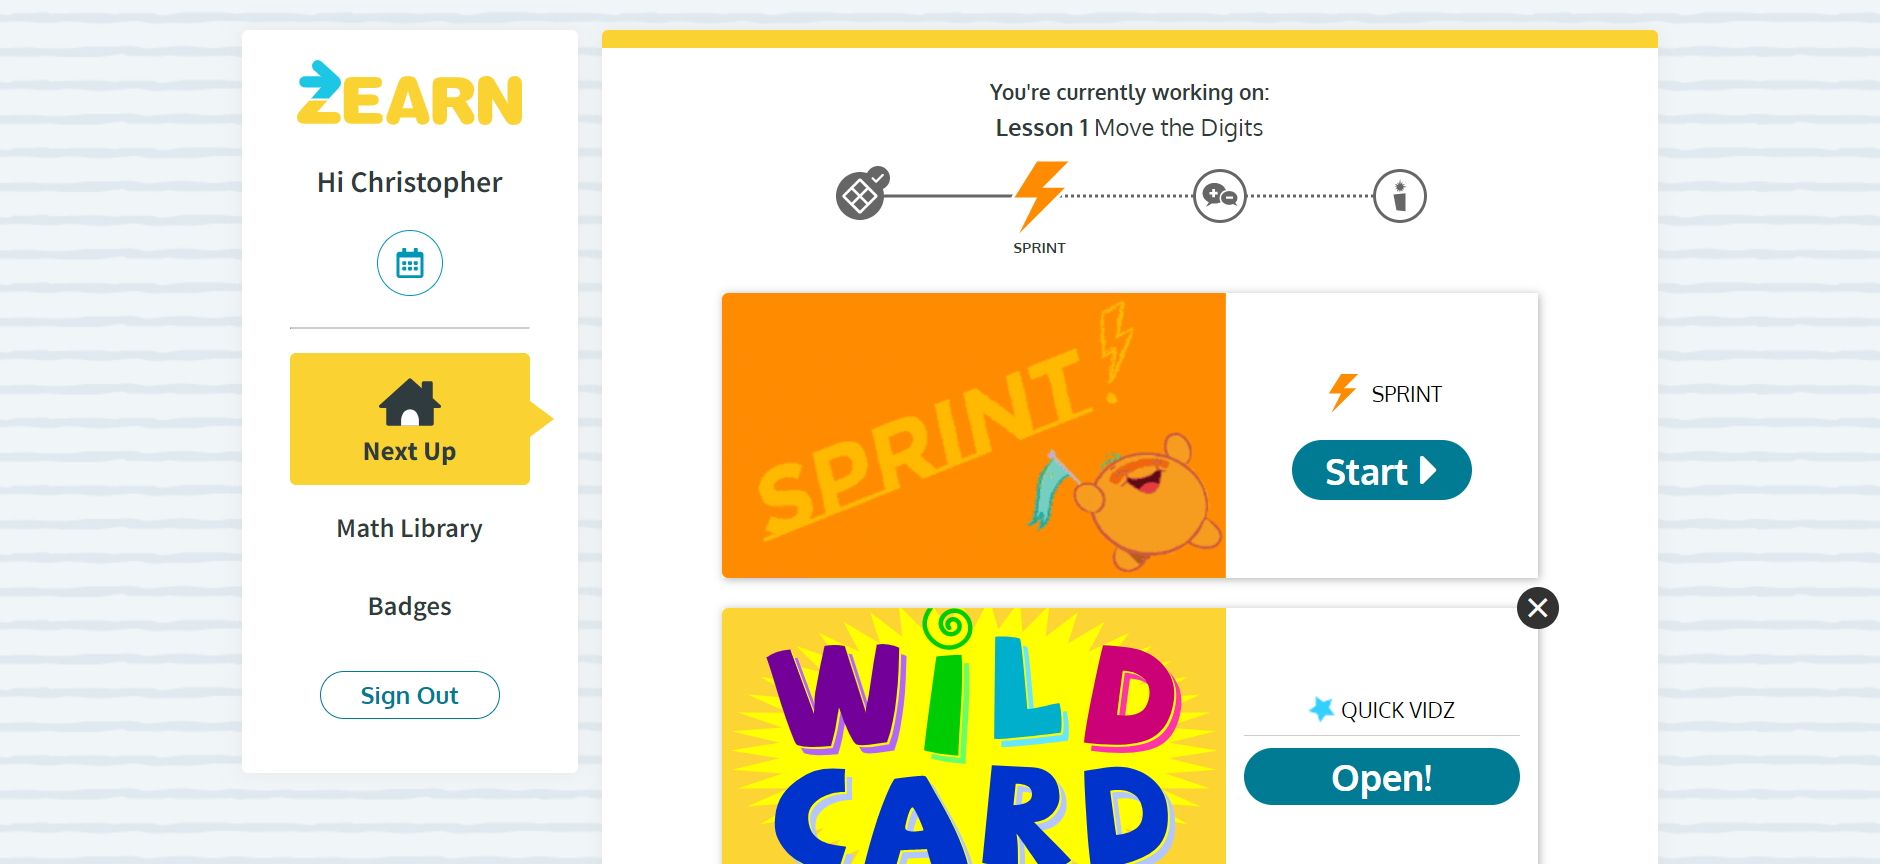
\includegraphics{images/student-feed.PNG}

}

\caption{\label{fig-st-portal}Zearn Student Portal}

\end{figure}

\begin{figure}

{\centering 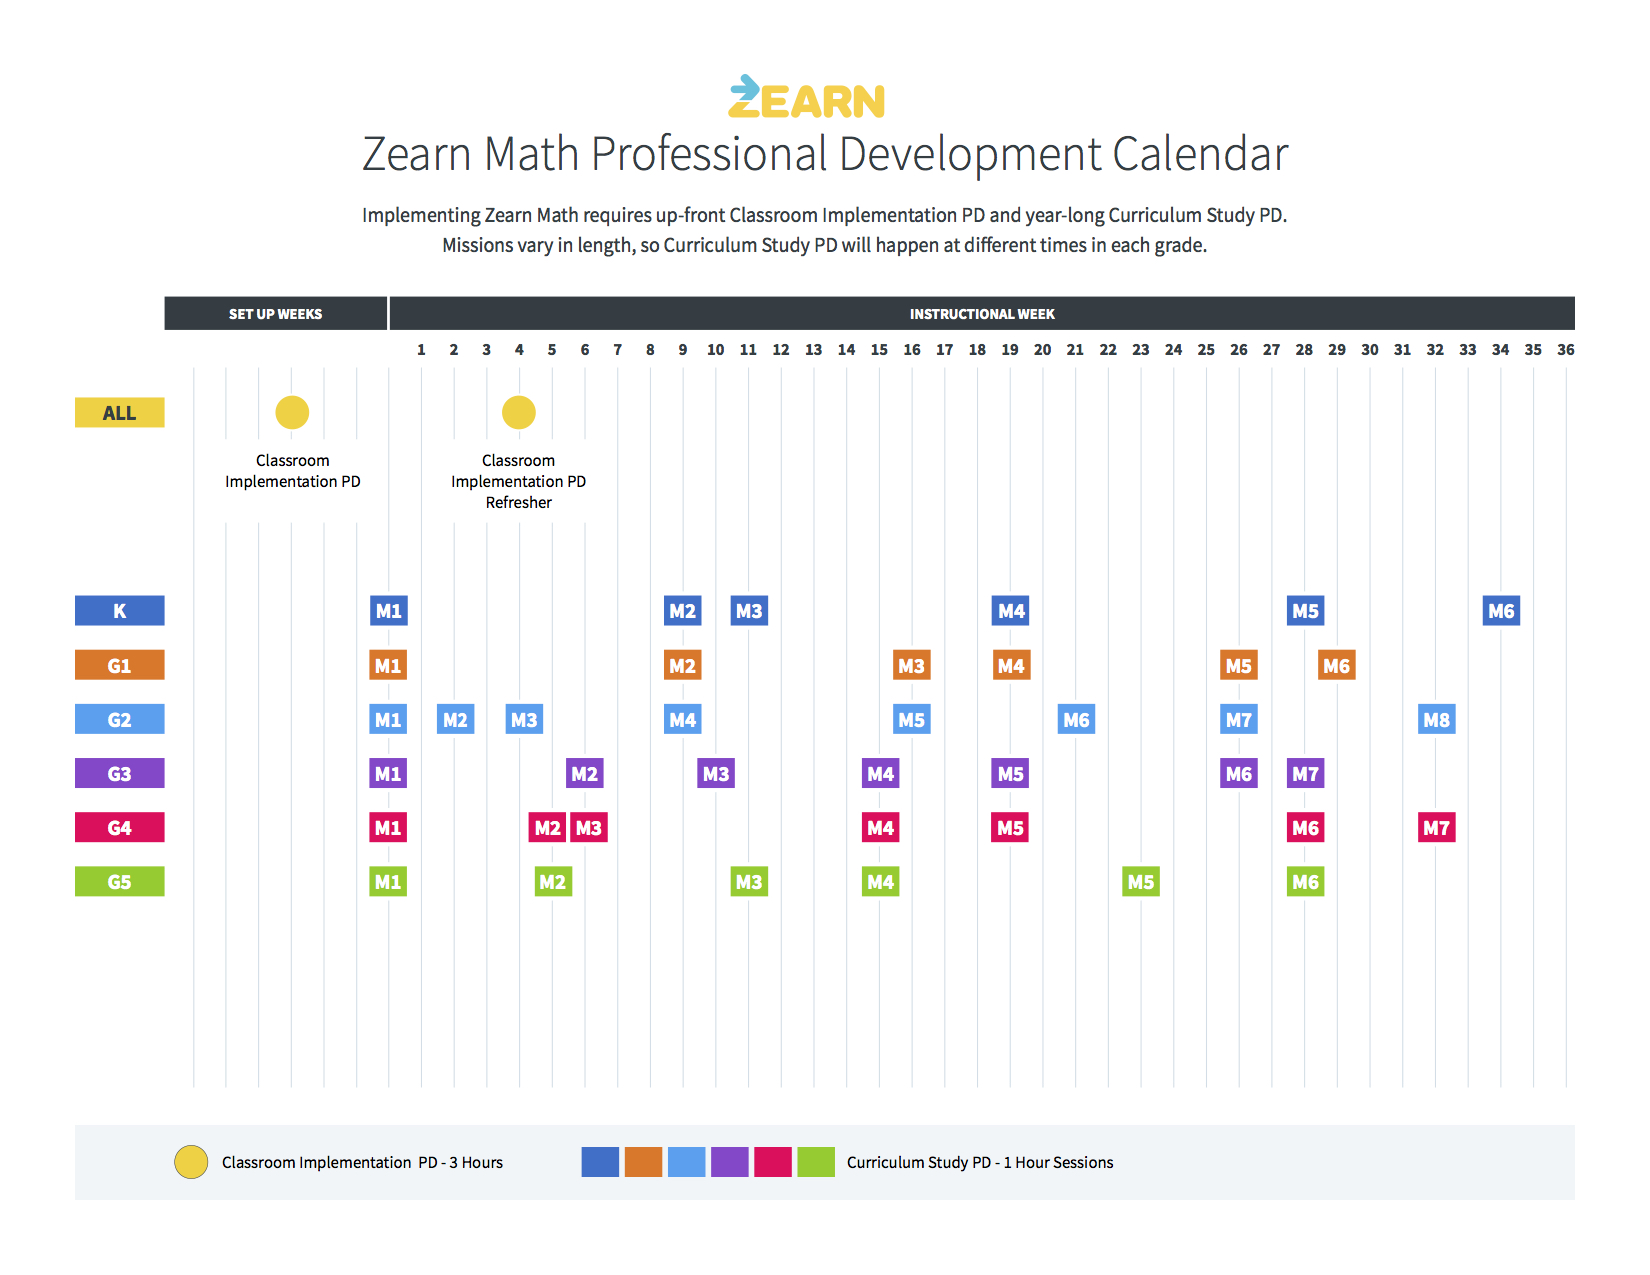
\includegraphics{images/PD-calendar.jpg}

}

\caption{\label{fig-prof-dev}Professional Development Calendar}

\end{figure}

\hypertarget{zearns-eye-view-of-the-data}{%
\subsection{Zearn's Eye View of the
Data}\label{zearns-eye-view-of-the-data}}

\hypertarget{pooled-correlations-between-components-and-student-outcomes}{%
\subsection{Pooled Correlations between Components and Student
Outcomes}\label{pooled-correlations-between-components-and-student-outcomes}}

We meta-analyzed individual correlations within our dataset to reveal
the pooled relationships between student outcomes (badges) and the
components from the dimensionality reduction procedure. This approach,
termed `internal meta-analysis,' is advantageous when dealing with large
datasets with hierarchical structures, as it allows for simultaneously
considering multiple, potentially correlated outcomes.

To conduct this internal meta-analysis, we first transformed the
correlations using Fisher's z-transformation, ensuring a normal
distribution of the correlations. We then ran a random effects model
with each unique combination of ``Teacher'' and ``School.'' This
multivariate meta-analysis offers the advantage of modeling multiple,
potentially correlated outcomes, providing a comprehensive estimate of
the correlations for each outcome, considering the hierarchical
structure of the data. The outcome of this process is a robust
understanding of the relationships between different outcomes and the
Badges across diverse schools and teachers. This approach provides a
more resilient analysis than simple correlations, as it accounts for the
inherent variability and dependencies within the data.
Figure~\ref{fig-meta-analysis} displays the results and illustrates the
pooled correlations between the components and student outcomes.

\begin{verbatim}
List of 2
 $ legend.position : num [1:2] 0.85 0.24
 $ legend.direction: chr "vertical"
 - attr(*, "class")= chr [1:2] "theme" "gg"
 - attr(*, "complete")= logi FALSE
 - attr(*, "validate")= logi TRUE
\end{verbatim}

\begin{figure}

{\centering \includegraphics{zearn_files/figure-pdf/fig-meta-analysis-1.pdf}

}

\caption{\label{fig-meta-analysis}Results of the correlation
meta-analysis.}

\end{figure}

\hypertarget{bayesian-model-diagnostics}{%
\subsection{Bayesian Model
Diagnostics}\label{bayesian-model-diagnostics}}

\begin{table}

\end{table}

\hypertarget{bayesian-model-estimates}{%
\subsection{Bayesian Model Estimates}\label{bayesian-model-estimates}}

This section presents the group parameter estimates for all
Reinforcement Learning (RL) models, both non-hierarchical and
hierarchical. To generate these group parameter estimates, we first
extract the posterior samples from the fitted models and calculate the
mean (M), standard deviation (SD), 25th percentile (Q1), and 75th
percentile (Q3) for each parameter. \textbf{?@tbl-group-parameters}
summarizes the distribution of the parameter estimates across
classrooms, revealing their typical values and variability.

\begin{table}

\end{table}




\end{document}
